% =============================================================================
%  Technický report: Biometrická autentifikácia podľa rytmu písania
% =============================================================================
%
%  AKO SA DOKUMENT PREKLADÁ
%    pdflatex main  ->  bibtex main  ->  pdflatex main  ->  pdflatex main
%    (v Overleafe stačí tlačidlo „Recompile“; hlavný súbor je main.tex)
%
%  ŠTRUKTÚRA PRIEČINKA
%    main.tex          tento súbor: nastavenia, titulná strana, poradie kapitol
%    sections/         jedna kapitola = jeden súbor (vkladajú sa cez \input)
%    figures/          obrázky (snímky obrazoviek)
%    references.bib    zoznam literatúry
%
%  POZOR: Zadanie vyžaduje šablónu LaTeX zverejnenú v tíme na MS Teams.
%  Tento súbor používa neutrálnu triedu `article`, aby sa dal skompilovať.
%  Postup: stiahnite si šablónu, jej preambulu a titulnú stranu použite
%  namiesto tých tu a obsah priečinka `sections/` len vložte pomocou \input.
% =============================================================================
\documentclass[11pt,a4paper]{article}


% -----------------------------------------------------------------------------
%  1. BALÍKY
% -----------------------------------------------------------------------------
% --- jazyk a kódovanie (slovenčina, diakritika, delenie slov) ---
\usepackage[utf8]{inputenc}           % vstupný súbor je v UTF-8
\usepackage[T1]{fontenc}              % správne písmená s diakritikou vo fonte
\usepackage[slovak]{babel}            % slovenské delenie slov a názvy (Obr., Tabuľka)
\usepackage{lmodern}                  % vektorový font Latin Modern

% --- rozloženie strany ---
\usepackage[margin=2.5cm]{geometry}   % okraje 2,5 cm
\usepackage{titlesec}                 % úpravy nadpisov kapitol
\newcommand{\sectionbreak}{\clearpage} % každá kapitola (1, 2, 3, ...) začína na novej strane
\usepackage{setspace}                 % riadkovanie
\usepackage{etoolbox}                 % \BeforeBeginEnvironment, \AfterEndEnvironment
\onehalfspacing                       % väčšie riadkovanie (1,5) kvôli čitateľnosti
\setlength{\parindent}{0pt}            % odseky bez odsadenia prvého riadku
\setlength{\parskip}{0.7em plus 0.2em} % namiesto odsadenia sa odseky oddelia malou medzerou

% --- obrázky, tabuľky, vzorce ---
\usepackage{graphicx}                 % \includegraphics
\usepackage{float}                    % [H] pre obrázky v príručke
\usepackage{booktabs}                 % pekné vodorovné čiary v tabuľkách (\toprule...)
\usepackage{tabularx}                 % tabuľky so stĺpcom roztiahnutým na šírku strany
\usepackage{amsmath}                  % matematické prostredia (equation, align)
\usepackage{caption}                  % nastavenie popisov (medzery pod/nad popisom)

% --- farby, výpisy kódu, schémy ---
\usepackage[table]{xcolor}            % farby + farebné riadky tabuliek (\rowcolor)
\usepackage{listings}                 % výpisy zdrojového kódu
\usepackage{tikz}                     % kreslenie schém priamo v LaTeXu
\usetikzlibrary{positioning,arrows.meta,shapes.geometric}

% --- odkazy v PDF (obsah, \ref, URL) bez farebných rámčekov ---
\usepackage[hidelinks]{hyperref}

% Obrázky sa hľadajú v priečinku figures/
\graphicspath{{figures/}}

% --- medzery okolo popisov a tabuliek -----------------------------------------
% Popis tabuľky je NAD tabuľkou, popis obrázka POD obrázkom. Štandardná trieda
% `article` nechá pod popisom nulovú medzeru, preto ju nastavujeme výslovne.
\captionsetup[table]{position=above, skip=10pt}    % popis tabuľky -> 10 pt -> tabuľka
\captionsetup[figure]{position=below, skip=8pt}    % obrázok -> 8 pt -> popis obrázka

% --- medzera medzi textom a obrázkom/tabuľkou ---------------------------------
% Platí pre všetky obrázky a tabuľky. Zväčšením čísla sa odsadia viac.
% (plus/minus = povolená pružnosť, aby sa strana dala pekne vyplniť)
\setlength{\intextsep}{22pt plus 4pt minus 4pt}    % obrázok/tabuľka v strede textu: nad aj pod ním
\setlength{\floatsep}{22pt plus 4pt minus 4pt}     % medzi dvoma plávajúcimi objektmi za sebou
\setlength{\textfloatsep}{24pt plus 4pt minus 4pt} % obrázok na začiatku/konci strany
% Popisy: rovnaký tvar „Tab. 1“ a „Obr. 1“ ako v texte aj v šablóne TUKE
\addto\captionsslovak{\renewcommand{\tablename}{Tab.}\renewcommand{\figurename}{Obr.}}

% --- plávajúce objekty: dovoľ ich umiestniť aj s textom, aby nezostávali samy na strane ---
\renewcommand{\topfraction}{0.9}
\renewcommand{\bottomfraction}{0.8}
\renewcommand{\textfraction}{0.1}
\renewcommand{\floatpagefraction}{0.75}
\setcounter{totalnumber}{4}

% --- tabuľky: všetky na celú šírku strany, so zvislými čiarami -------------------
% Y = text zarovnaný vľavo, C = text na stred; obe vyplnia zvyšnú šírku tabuľky.
% M{šírka} = stĺpec pevnej šírky, text na stred.
\newcolumntype{Y}{>{\raggedright\arraybackslash}X}
\newcolumntype{C}{>{\centering\arraybackslash}X}
\newcolumntype{M}[1]{>{\centering\arraybackslash}p{#1}}
\renewcommand{\arraystretch}{1.35}   % výška riadkov (1.0 = tesné)
\setlength{\tabcolsep}{7pt}          % vodorovný okraj v bunke


% -----------------------------------------------------------------------------
%  2. VLASTNÉ PRÍKAZY
% -----------------------------------------------------------------------------
% \todo{text}  -> červená tučná značka na mieste, ktoré treba ešte doplniť.
%                Pred odovzdaním v PDF vyhľadajte „DOPLNIŤ“ a všetky odstráňte.
\newcommand{\todo}[1]{\textbf{\textcolor{red}{[DOPLNIŤ: #1]}}}

% \code{text}  -> neproporcionálne písmo pre názvy súborov, príkazov a polí.
%                Podčiarkovník v texte píšte ako \_ (napr. \code{participant\_id}).
\newcommand{\code}[1]{\texttt{#1}}

% Vzhľad výpisov kódu (prostredie lstlisting)
% Slovenské znaky sa v kóde prepisujú cez `literate`, aby fungovali komentáre
% s diakritikou. Pre Python sa pri výpise pridáva [language=Python].
\lstset{
  basicstyle=\ttfamily\small,                      % písmo kódu
  keywordstyle=\color{blue!60!black}\bfseries,     % kľúčové slová
  commentstyle=\color{green!35!black}\itshape,     % komentáre: zelená kurzíva
  stringstyle=\color{red!50!black},                % reťazce
  showstringspaces=false,
  backgroundcolor=\color{gray!8},                  % jemné pozadie výpisu
  frame=single, rulecolor=\color{gray!60},         % rámček
  framesep=8pt,                                    % vnútorný okraj rámčeka
  framerule=0.6pt,
  xleftmargin=8.6pt, xrightmargin=8.6pt,           % = framesep + framerule: rámček má šírku textu ako tabuľky
  aboveskip=1.5em, belowskip=1.3em,                % medzera nad a pod výpisom
  lineskip=3pt,                                    % medzera medzi riadkami kódu
  tabsize=4,
  breaklines=true, breakatwhitespace=true,         % dlhé riadky sa zalomia
  columns=fullflexible, keepspaces=true,
  extendedchars=true, inputencoding=utf8,
  literate=
    {á}{{\'a}}1 {é}{{\'e}}1 {í}{{\'i}}1 {ó}{{\'o}}1 {ú}{{\'u}}1 {ý}{{\'y}}1
    {č}{{\v c}}1 {ď}{{\v d}}1 {ľ}{{\v l}}1 {ň}{{\v n}}1 {š}{{\v s}}1 {ť}{{\v t}}1 {ž}{{\v z}}1
    {ä}{{\"a}}1 {ô}{{\^o}}1 {ĺ}{{\'l}}1 {ŕ}{{\'r}}1
    {Á}{{\'A}}1 {É}{{\'E}}1 {Í}{{\'I}}1 {Ó}{{\'O}}1 {Ú}{{\'U}}1 {Ý}{{\'Y}}1
    {Č}{{\v C}}1 {Ď}{{\v D}}1 {Ľ}{{\v L}}1 {Ň}{{\v N}}1 {Š}{{\v S}}1 {Ť}{{\v T}}1 {Ž}{{\v Z}}1
    {Ä}{{\"A}}1 {Ô}{{\^O}}1,
}

% Výpis kódu sa nikdy nelomí medzi dve strany: celý výpis je vložený do
% minipage (neprerušiteľný blok), takže ak sa nezmestí na stranu, presunie sa
% celý na ďalšiu. Samotné prostredie samepage rámček výpisu nezabránilo
% rozdeliť (na novej strane zostal prázdny pás s dolným okrajom rámčeka).
% Platí pre výpisy kratšie ako strana; dlhší výpis by tu pretiekol cez okraj.
\BeforeBeginEnvironment{lstlisting}{\par\nopagebreak[4]\noindent\begin{minipage}{\linewidth}}
\AfterEndEnvironment{lstlisting}{\end{minipage}\par}

% Metadáta PDF súboru
\hypersetup{
  pdftitle={Biometrická autentifikácia podľa rytmu písania},
  pdfauthor={Tetiana Mohorian, Artem Skrypnyk, Polina Istomina},
}


% -----------------------------------------------------------------------------
%  3. PRÍKAZY PRE TITULNÚ STRANU
%     Rozloženie podľa šablóny TUKE (Word). Údaje sa menia tu, nie v texte strany.
% -----------------------------------------------------------------------------
% Hlavička: univerzita a fakulta
\newcommand{\tukeheader}{%
  {\bfseries\LARGE TECHNICKÁ UNIVERZITA V~KOŠICIACH\par}
  \vspace{0.8em}
  {\bfseries\Large FAKULTA ELEKTROTECHNIKY A~INFORMATIKY\par}}

% Názov práce a jej druh
\newcommand{\worktitle}{%
  {\bfseries\LARGE BIOMETRICKÁ AUTENTIFIKÁCIA\\PODĽA RYTMU PÍSANIA\par}
  \vspace{0.8em}
  {\bfseries\large Semestrálne zadanie -- technický report\par}}

% Zoznam autorov (každý na vlastnom riadku)
\newcommand{\authorlines}{Bc.\ Tetiana Mohorian\\ Bc.\ Artem Skrypnyk\\ Bc.\ Polina Istomina}

% Pätička titulnej strany: vľavo text (#1, napr. rok), vpravo autori
\newcommand{\titlefooter}[1]{%
  \noindent\begin{minipage}[b]{0.4\textwidth}\raggedright\bfseries\large #1\end{minipage}%
  \hfill
  \begin{minipage}[b]{0.55\textwidth}\raggedleft\bfseries\large \authorlines\end{minipage}}


% =============================================================================
%  4. DOKUMENT
% =============================================================================
\begin{document}

% --- titulná strana (obálka): hlavička hore, názov v strede, rok a autori dole ---
\begin{titlepage}
  \centering
  \tukeheader
  \vspace*{\fill}               % pružná medzera: názov sa vycentruje
  \worktitle
  \vspace*{\fill}
  \titlefooter{\the\year}       % \the\year = aktuálny rok pri preklade
\end{titlepage}

% --- obsah (generuje sa z \section a \subsection; prekladajte dvakrát) ---
% Obsah je jednoriadkový, aby sa zmestil na jednu stranu aj pri väčšom riadkovaní textu.
\begin{singlespace}
\setlength{\parskip}{0pt}                 % bez medzier medzi riadkami obsahu
\tableofcontents
\end{singlespace}

% --- zoznam obrázkov, zoznam tabuliek a zoznam symbolov a skratiek (ako v šablóne TUKE) ---
% Každý zoznam začína na novej strane (\sectionbreak z preambuly) a je aj v obsahu.
\clearpage
\addcontentsline{toc}{section}{\listfigurename}
\begin{singlespace}
\setlength{\parskip}{0pt}
\listoffigures
\end{singlespace}

\clearpage
\addcontentsline{toc}{section}{\listtablename}
\begin{singlespace}
\setlength{\parskip}{0pt}
\listoftables
\end{singlespace}

\clearpage
\section*{Zoznam symbolov a skratiek}
\addcontentsline{toc}{section}{Zoznam symbolov a skratiek}

\begin{singlespace}
\small
\renewcommand{\arraystretch}{1.25}
\setlength{\parskip}{0pt}

\subsection*{Symboly}
\begin{tabularx}{\textwidth}{@{}>{\bfseries}p{3.2cm}Y@{}}
  \toprule
  $n$ & počet kláves v jednom pokuse (37 pre vetu, 10 pre slovo) \\
  $m$ & počet príznakov jedného pokusu, $m = 2n-1$ \\
  $h_i$ & doba držania $i$-tej klávesy \\
  $g_i$ & interval medzi $i$-tym a $(i+1)$-vým stlačením \\
  $\mathbf{x}$ & vektor príznakov pokusu \\
  $\boldsymbol{\mu}$, $\boldsymbol{\sigma}$ & priemer a smerodajná odchýlka príznakov v šablóne \\
  $d(\mathbf{x}, P)$ & štandardizovaná vzdialenosť pokusu od šablóny $P$ \\
  $p_i$ & relatívna miera podobnosti $i$-teho z troch najbližších účastníkov \\
  \bottomrule
\end{tabularx}

\subsection*{Skratky}
\begin{tabularx}{\textwidth}{@{}>{\bfseries}p{3.2cm}Y@{}}
  \toprule
  API & rozhranie na programovanie aplikácií \\
  CNN, GRU & konvolučná a rekurentná neurónová sieť \\
  CSV & textový formát s hodnotami oddelenými čiarkou \\
  EER & chybovosť, pri ktorej sa rovnajú nesprávne prijatia a nesprávne odmietnutia \\
  FAR, FRR & podiel prijatých cudzích a podiel odmietnutých vlastných pokusov \\
  GDPR & všeobecné nariadenie EÚ o ochrane osobných údajov \\
  HTTP & protokol na prenos dát medzi klientom a serverom \\
  JSON & textový formát na výmenu dát \\
  REST & štýl návrhu webového rozhrania cez HTTP \\
  SQL & jazyk na prácu s databázou \\
  top-$k$ & podiel pokusov, pri ktorých je správny účastník medzi $k$ najpodobnejšími \\
  \bottomrule
\end{tabularx}
\end{singlespace}
% (nová strana pred prvou kapitolou zabezpečuje \sectionbreak z preambuly)

% --- kapitoly: poradie tu určuje poradie v dokumente ---
\section{Úvod}

Dynamika písania (angl.\ \emph{keystroke dynamics}) je behaviorálna biometria,
ktorá z času stlačenia a uvoľnenia kláves odvodzuje charakteristický rytmus
písania konkrétneho človeka. Nepotrebuje špeciálny hardvér, stačí bežná
klávesnica, a dá sa vyhodnocovať počas písania.

Cieľom tejto práce je navrhnúť, implementovať a otestovať jednoduchý systém,
ktorý (i) zbiera časy stlačenia kláves od účastníkov experimentu pri písaní
tej istej vety a (ii) z jedného nového pokusu určí, ktorému z už známych
účastníkov sa rytmus písania najviac podobá. Riešenie pozostáva z webovej
aplikácie na zber dát, serverovej časti s úložiskom a algoritmu na
identifikáciu. Zdrojový kód je dostupný v repozitári~\cite{repo}.

Dokument je členený takto: kapitola~\ref{sec:teoria} zhŕňa teoretické
východiská, kapitola~\ref{sec:navrh} opisuje návrh riešenia a použitú metódu,
kapitola~\ref{sec:impl} implementáciu, kapitola~\ref{sec:test} testovanie
a vyhodnotenie a kapitola~\ref{sec:prirucka} slúži ako príručka na spustenie
a používanie systému.
              % 1 Úvod
\section{Teoretické východiská}
\label{sec:teoria}

% Kapitola vychádza z odbornej literatúry (zdroje sú v references.bib).
% Rozsah má byť najviac 3 strany. Pred odovzdaním skontrolujte, že každé
% tvrdenie zodpovedá obsahu citovaného zdroja.

\subsection{Behaviorálna biometria}

Biometrická autentifikácia overuje alebo určuje totožnosť človeka podľa jeho
telesných alebo behaviorálnych vlastností. Behaviorálna biometria vychádza zo
spôsobu, akým človek koná, a dynamika písania na klávesnici patrí k jej
najľahšie dostupným podobám: nepotrebuje špeciálny snímač, stačí bežná
klávesnica a údaje sa dajú zbierať počas písania~\cite{roy2022,shadman2023}.
Prehľad aktuálnej literatúry poskytuje systematický prehľad zameraný na
modely dynamiky písania z rokov 2017 až 2022~\cite{roy2022}, ktorý porovnáva
použité metódy, nastavenia experimentov aj otvorené problémy, a prehľadová
štúdia o pojmoch, technikách a aplikáciách, ktorá sa venuje aj dátovým súborom,
písaniu na dotykových zariadeniach a použitiu mimo autentifikácie~\cite{shadman2023}.

Rozlišujú sa dve úlohy: \emph{verifikácia} (overenie, že človek je tým, za koho
sa vydáva) a \emph{identifikácia} (určenie, ktorému zo známych ľudí sa
záznam najviac podobá). Táto práca rieši identifikáciu. Podľa typu písaného
textu sa ďalej rozlišuje písanie \emph{pevného} textu (všetci píšu to isté,
ako v tejto práci) a písanie \emph{voľného} textu, ktoré umožňuje priebežné
overovanie počas bežnej práce na počítači~\cite{shadman2023}.

\subsection{Príznaky dynamiky písania}

Základom sú časy stlačenia a uvoľnenia klávesov. Z nich sa odvádzajú dva
druhy príznakov: doba držania klávesy (čas medzi stlačením a uvoľnením)
a intervaly medzi po sebe idúcimi klávesmi, ktoré sa v literatúre nazývajú aj
letové časy (\emph{flight time})~\cite{kaluarachchi2023}. Autori práce o súbore
DEFT ukazujú, že doplnenie letových časov o vzdialenosť medzi klávesmi
vytvára príznakovú množinu nezávislú od zariadenia,
s presnosťou nad 99\,\% a chybovosťou EER pod 10\,\% na troch zariadeniach~\cite{kaluarachchi2023}.
Zaujímavým zistením je, že aj príznaky založené len na časoch, bez znalosti
obsahu textu, si zachovávajú uspokojivý výkon pri verifikácii~\cite{stragapede2023}.
Práve takéto časové príznaky (doby držania a intervaly) používa aj riešenie
v tejto práci (podkapitola~\ref{sec:priznaky}).

\subsection{Metódy vyhodnotenia}

Pri klasifikácii sa používajú jednoduché štatistické miery vzdialenosti aj
metódy strojového učenia. Porovnanie klasických algoritmov strojového učenia
a techník výberu príznakov (filtrovacích a obalových) na úlohe autentifikácie
podľa dynamiky písania uvádza štúdia~\cite{teotia2023}. Pri voľnom texte sa
úspešne používajú aj hlboké neurónové siete: rekurentná sieť TypeNet
dosiahla chybovosť EER 2,2\,\% na fyzickej klávesnici a 9,2\,\% na dotykovej
a pri nárasti počtu používateľov až do 100\,000 sa chyba zvýšila len mierne~\cite{acien2021},
a kombinácia konvolučnej a rekurentnej siete (CNN a GRU) dosiahla na voľnom
texte výsledky porovnateľné s najlepšími predchádzajúcimi prístupmi~\cite{chang2021}.
Autori porovnania z roku 2026 zdôrazňujú, že výsledky veľmi závisia od výberu
dátového súboru a spôsobu vyhodnotenia, že hlboké učenie vedie pri voľnom texte
a že tvrdenia o kvantových prístupoch zatiaľ nie sú podložené~\cite{gundogan2026}.
Aj preto vznikla verejná výzva KVC, ktorá porovnáva systémy na rovnakých dátach
a okrem presnosti hodnotí aj spravodlivosť voči demografickým skupinám~\cite{stragapede2023}.

Verifikačné systémy sa najčastejšie hodnotia mierou EER (\emph{equal error
rate}), teda chybovosťou, pri ktorej je podiel nesprávne prijatých pokusov
rovnaký ako podiel nesprávne odmietnutých~\cite{acien2021,stragapede2023}.
Pri identifikácii na malom počte ľudí je
prirodzenejšie sledovať, či je správny človek na prvom mieste (top-1) alebo
medzi prvými $k$ (top-$k$); tieto metriky používa aj táto práca
(podkapitola~\ref{sec:protokol}). Nie sú priamo porovnateľné s EER, preto sa
výsledky tejto práce nedajú jednoducho porovnávať s číslami z citovaných
štúdií, ktoré používajú iné dáta a iný protokol.

\subsection{Súkromie a ochrana osobných údajov}

Dynamika písania je citlivý údaj. Behaviorálne príznaky môžu prezradiť aj
pohlavie, vek, dominantnú ruku či emocionálny stav písajúceho~\cite{baig2022},
a preto sa navrhujú protokoly, v ktorých server nikdy nevidí biometrické šablóny
v otvorenej podobe, napríklad s využitím homomorfného šifrovania~\cite{baig2022}.
Pri právnom posúdení treba brať do úvahy, že terminológia GDPR rozlišuje
rozpoznávanie osoby a len klasifikáciu jej vlastností (napríklad tzv. mäkkých
znakov) a že druhý prípad je chránený menej, čo vytvára riziká pre súkromie~\cite{bisztray2021}. Tieto
úvahy sú dôvodom, prečo sa pri zbere údajov v tejto práci uplatňuje informovaný
súhlas, minimalizácia údajov a lokálne úložisko (podkapitola~\ref{sec:etika}).
            % 2 Teoretické východiská
\section{Návrh riešenia}
\label{sec:navrh}

% ----- Požiadavky -----
\subsection{Požiadavky}

Systém musí spĺňať tieto požiadavky:
% Odrážkový zoznam.
\begin{itemize}
  \item zaznamenať pre každé stlačenie klávesy čas stlačenia aj uvoľnenia
        s rozlíšením lepším ako milisekunda,
  \item zabezpečiť, aby všetci účastníci písali tú istú vetu rovnakým
        spôsobom (bez opráv a bez vkladania textu),
  \item uložiť namerané údaje v tvare vhodnom na ďalšie spracovanie,
  \item z jedného nového pokusu určiť najpodobnejších účastníkov a posúdiť,
        či ide o neznámu osobu,
  \item umožniť vyhodnotenie úspešnosti na dátach, ktoré neboli použité
        na tvorbu šablón.
\end{itemize}

% ----- Architektúra -----
\subsection{Architektúra}

Riešenie má dve časti (Obr.~\ref{fig:arch}). Webová aplikácia
(klient) beží v prehliadači, zaznamenáva klávesové udalosti a zobrazuje
výsledky. Serverová časť (REST API) ukladá relácie do databázy SQLite
a obsahuje algoritmus identifikácie. Komunikácia prebieha vo formáte JSON
cez HTTP.

% Obrázok (schéma nakreslená v TikZ): Architektúra systému.
\begin{figure}[ht]
  \centering
  \vspace{1.5em}   % <- prázdny riadok (medzera) medzi textom hore a schémou; zmeňte číslo podľa potreby
  \begin{tikzpicture}[
      box/.style={draw, rounded corners=4pt, thick, minimum width=3.4cm, minimum height=1.9cm,
                  align=center, fill=gray!10},
      lbl/.style={font=\small, align=center, inner sep=2pt},
      cap/.style={font=\footnotesize\itshape, text=gray},
      >={Stealth[length=3mm]}, node distance=2.6cm]
    % tri bloky vedľa seba: klient -> server -> databáza
    \node[box] (ui)  {\textbf{Webová aplikácia}\\[3pt]\small React, prehliadač};
    \node[box, right=of ui]  (api) {\textbf{REST API}\\[3pt]\small FastAPI, Python};
    \node[box, right=of api] (db)  {\textbf{Databáza}\\[3pt]\small SQLite};
    % šípky v oboch smeroch (požiadavka a odpoveď)
    \draw[<->, thick] (ui) -- node[above, lbl] {JSON\\cez HTTP} (api);
    \draw[<->, thick] (api) -- node[above, lbl] {SQL} (db);
    % popisky pod blokmi
    \node[cap, below=4pt of ui]  {klient};
    \node[cap, below=4pt of api] {server};
    \node[cap, below=4pt of db]  {úložisko};
  \end{tikzpicture}
  \caption{Architektúra systému.}
  \label{fig:arch}
\end{figure}

Klient pracuje v štyroch stavoch: príprava relácie, meranie, identifikácia
jedného pokusu a záverečná obrazovka s možnosťou odoslať dáta na server.

% ----- Zber údajov -----
\subsection{Zber údajov}

Účastník zadá meno, vyberie zariadenie (notebook alebo stolný počítač)
a typ klávesnice (vstavaná, externá USB, externá Bluetooth) a vyjadrí súhlas
so záznamom. Následne \textbf{15-krát} napíše vetu
\emph{„Every keystroke tells a unique story.“} (37 znakov) a každý pokus
potvrdí klávesom Enter.

Na meranie času sa používa \code{performance.now()}. Čas každej udalosti sa
ukladá relatívne k prvému stlačeniu v danom pokuse. Klávesy Shift, Caps Lock,
Ctrl, Alt, Meta, Tab a Escape sa nezaznamenávajú. Opakované udalosti pri
podržaní klávesy sa blokujú. Vkladanie, vystrihovanie, presúvanie textu
a kontextové menu sú vo vstupnom poli zakázané.

Pokus sa zamietne a účastník ho musí zopakovať, ak:
% Odrážkový zoznam.
\begin{itemize}
  \item napísaný text sa nezhoduje s vetou,
  \item počet stlačení sa líši od počtu uvoľnení (nie všetky klávesy boli
        uvoľnené).
\end{itemize}
Na strane servera sa navyše pri vytváraní šablón ignoruje každý pokus,
ktorý nemá presne 37 stlačení a 37 uvoľnení (podkapitola~\ref{sec:priznaky}).

% ----- Formát údajov -----
\subsection{Formát údajov}

Každá klávesová udalosť je jeden riadok s poľami uvedenými v
Tab.~\ref{tab:format}. Relácia sa na server odosiela ako objekt
\code{\{meta, rows\}}, kde \code{meta} obsahuje identifikáciu účastníka
a relácie a \code{rows} zoznam udalostí všetkých pokusov.

% Tabuľka: Polia záznamu o klávesovej udalosti.
\begin{table}[ht]
  \centering
  \small
  \caption{Polia záznamu o klávesovej udalosti.}
  \label{tab:format}
  \begin{tabularx}{\textwidth}{|l|Y|}
    \hline
    \rowcolor[gray]{0.9} \textbf{Pole} & \textbf{Význam} \\
    \hline
    \code{participant\_id} & identifikátor účastníka (zadané meno) \\
    \hline
    \code{session\_id} & čas začiatku relácie vo formáte ISO 8601 \\
    \hline
    \code{device}, \code{keyboard} & zariadenie a typ klávesnice \\
    \hline
    \code{rep} & poradové číslo pokusu (1--15) \\
    \hline
    \code{seq} & poradie udalosti v rámci pokusu \\
    \hline
    \code{event} & \code{down} (stlačenie) alebo \code{up} (uvoľnenie) \\
    \hline
    \code{code}, \code{key} & fyzický kód klávesy a vyprodukovaný znak \\
    \hline
    \code{t\_ms} & čas v ms od prvého stlačenia v pokuse \\
    \hline
  \end{tabularx}
\end{table}

% ----- Príznaky -----
\subsection{Príznaky}
\label{sec:priznaky}

Z jedného pokusu s $n=37$ klávesmi sa vytvorí vektor príznakov. Nech $d_i$ je
čas $i$-teho stlačenia a $u_i$ čas uvoľnenia tej istej klávesy (prvá udalosť
\code{up} s rovnakým \code{code}, ktorá nasleduje po stlačení). Potom platia
vzorce~\eqref{eq:hold} a~\eqref{eq:gap}:
% Vzorec (v texte sa číta ako matematický zápis).
\begin{align}
  h_i &= u_i - d_i, & i &= 1,\dots,n, \label{eq:hold}\\
  g_i &= d_{i+1} - d_i, & i &= 1,\dots,n-1, \label{eq:gap}
\end{align}
kde $h_i$ je doba držania klávesy (vzorec~\eqref{eq:hold}) a $g_i$ interval medzi
dvoma po sebe idúcimi stlačeniami (vzorec~\eqref{eq:gap}). Vektor príznakov
$\mathbf{x} = (h_1,\dots,h_n,g_1,\dots,g_{n-1})$
má $m = 2n-1 = 73$ zložiek. Pokus s iným počtom stlačení či uvoľnení,
s chýbajúcim uvoľnením, nečíselným alebo záporným časom je neplatný.

% ----- Šablóna účastníka a miera podobnosti -----
\subsection{Šablóna účastníka a miera podobnosti}

Šablóna účastníka $P$ je dvojica vektorov $(\boldsymbol{\mu}, \boldsymbol{\sigma})$,
ktoré sa vypočítajú ako priemer a smerodajná odchýlka (populačná,
$\mathrm{ddof}=0$) jednotlivých príznakov z pokusov č.~1 až 10 všetkých
relácií daného účastníka. Ak je odchýlka príznaku nulová, nahradí sa
hodnotou 1, aby sa predišlo deleniu nulou.

Vzdialenosť nového pokusu $\mathbf{x}$ od šablóny $P$ je štandardizovaná
euklidovská vzdialenosť
% Vzorec (v texte sa číta ako matematický zápis).
\begin{equation}
  \label{eq:dist}
  d(\mathbf{x}, P) = \sqrt{\sum_{j=1}^{m}\left(\frac{x_j-\mu_j}{\sigma_j}\right)^{2}}.
\end{equation}
Vo vzorci~\eqref{eq:dist} je $m$ počet príznakov a $\mu_j$, $\sigma_j$ sú priemer
a smerodajná odchýlka $j$-teho príznaka v šablóne.
Účastníci sa zoradia podľa vzdialenosti vzostupne. Pokus sa označí ako
\emph{neznámy}, ak pre najbližšieho účastníka platí
% Vzorec (v texte sa číta ako matematický zápis).
\begin{equation}
  \label{eq:unknown}
  \frac{d_{\min}}{\sqrt{m}} > 3,
\end{equation}
Podmienka~\eqref{eq:unknown} znamená, že priemerná štandardizovaná odchýlka na jeden
príznak je väčšia ako tri.
Prah 3 je zvolený empiricky a nebol kalibrovaný na dátach.

Pre troch najbližších účastníkov sa vypočíta relatívna miera podobnosti
% Vzorec (v texte sa číta ako matematický zápis).
\begin{equation}
  \label{eq:share}
  p_i = 100\cdot\frac{w_i}{\sum_{k=1}^{3} w_k}, \qquad w_i = \frac{1}{d_i + 10^{-9}}.
\end{equation}
Hodnota $p_i$ zo vzorca~\eqref{eq:share} vyjadruje len relatívne poradie medzi tromi najlepšími
kandidátmi, \textbf{nie pravdepodobnosť}, že ide o danú osobu.

% ----- Číselný príklad výpočtu -----
\subsection{Číselný príklad výpočtu}
\label{sec:priklad}

Postup z predchádzajúcich podkapitol je ilustrovaný na zjednodušenom príklade
s tromi klávesmi. V skutočnom pokuse je $n=37$ a vektor má 73 zložiek,
tu je $n=3$ a vektor má $m=2n-1=5$ zložiek. Všetky hodnoty sú vymyslené
a slúžia len na vysvetlenie.

Pokus obsahuje udalosti z Tab.~\ref{tab:priklad-udalosti}.

% Tabuľka: Ilustračný pokus s tromi klávesmi (časy v ms).
\begin{table}[ht]
  \centering
  \small
  \caption{Ilustračný pokus s tromi klávesmi (časy v ms).}
  \label{tab:priklad-udalosti}
  \begin{tabularx}{\textwidth}{|C|C|C|C|}
    \hline
    \rowcolor[gray]{0.9} \textbf{Klávesa} & \textbf{Stlačenie $d_i$} & \textbf{Uvoľnenie $u_i$} & \textbf{Držanie $h_i=u_i-d_i$} \\
    \hline
    1 & 0 & 95 & 95 \\
    \hline
    2 & 140 & 230 & 90 \\
    \hline
    3 & 310 & 385 & 75 \\
    \hline
  \end{tabularx}
\end{table}

Intervaly medzi stlačeniami sú $g_1 = 140-0 = 140$ a $g_2 = 310-140 = 170$,
teda $\mathbf{x} = (95, 90, 75, 140, 170)$.

Nech šablóna účastníka obsahuje priemery a smerodajné odchýlky
$\boldsymbol{\mu} = (100, 90, 80, 150, 160)$ a
$\boldsymbol{\sigma} = (10, 10, 5, 20, 20)$. Štandardizované odchýlky sú
% Vzorec (v texte sa číta ako matematický zápis).
\[
  z_j = \frac{x_j-\mu_j}{\sigma_j} = (-0{,}5;\ 0;\ -1;\ -0{,}5;\ 0{,}5),
\]
a po dosadení do vzorca~\eqref{eq:dist} vzdialenosť
% Vzorec (v texte sa číta ako matematický zápis).
\[
  d = \sqrt{0{,}25 + 0 + 1 + 0{,}25 + 0{,}25} = \sqrt{1{,}75} \approx 1{,}323 .
\]
Pre kontrolu neznámeho pokusu podľa vzorca~\eqref{eq:unknown} je
$d/\sqrt{m} = 1{,}323/\sqrt{5} \approx 0{,}592$, čo je výrazne menej ako
prah 3, takže pokus sa neoznačí ako neznámy.

Ak by boli vzdialenosti od šablón troch účastníkov $d_1 \approx 1{,}323$,
$d_2 = 2{,}0$ a $d_3 = 4{,}0$, váhy sú $w_i = 1/d_i$ približne
$0{,}756$; $0{,}5$ a $0{,}25$ a relatívne miery podobnosti podľa vzorca~\eqref{eq:share}
$p_1 \approx 50{,}2\,\%$, $p_2 \approx 33{,}2\,\%$ a $p_3 \approx 16{,}6\,\%$.
Najbližší účastník má teda najvyššie percento, no hodnota 50,2\,\% neznamená,
že pravdepodobnosť zhody je 50,2\,\%.

% ----- Osobné údaje a etika zberu -----
\subsection{Osobné údaje a etika zberu}
\label{sec:etika}

Dynamika písania je biometrický údaj, ktorý môže jednoznačne súvisieť
s konkrétnou osobou, a preto sa so zozbieranými dátami zaobchádza ako
s osobnými údajmi. V systéme sa uplatňujú tieto zásady:
% Odrážkový zoznam.
\begin{itemize}
  \item \textbf{Informovaný súhlas.} Meranie sa nedá spustiť bez zaškrtnutia
        súhlasu so záznamom časových údajov stlačenia kláves na výskumné
        účely.
  \item \textbf{Minimalizácia údajov.} Zaznamenávajú sa len časy stlačenia
        a uvoľnenia kláves jednej vopred určenej vety. Obsah písaného textu
        je pre všetkých rovnaký a neobsahuje súkromné informácie. Okrem
        mena (identifikátora účastníka) sa ukladá len typ zariadenia
        a klávesnice.
  \item \textbf{Identifikátor účastníka.} Aplikácia vyžaduje meno
        a priezvisko, ktoré sa používa ako \code{participant\_id}. Databáza
        teda obsahuje osobné údaje a nemá sa zverejňovať.
  \item \textbf{Lokálne úložisko.} Dáta sa ukladajú do súboru SQLite
        na serveri riešenia; nepoužívajú sa žiadne externé služby.
  \item \textbf{Zdieľanie kódu bez dát.} Do repozitára patrí kód, nie
        databáza.
\end{itemize}

Na zverejnenie alebo odovzdanie dát tretím osobám treba zvážiť, či účastníci
s takým použitím súhlasili. Tento dokument nepredstavuje právne posúdenie.

% ----- Protokol vyhodnotenia -----
\subsection{Protokol vyhodnotenia}
\label{sec:protokol}

Aby sa šablóny neotestovali na tých istých dátach, z ktorých vznikli, sa
pokusy rozdelia podľa poradia: pokusy 1--10 slúžia na tvorbu šablóny,
pokusy 11--15 na testovanie. Pre každý testovací pokus sa zistí poradie
účastníkov a vyhodnotia sa:
% Odrážkový zoznam.
\begin{itemize}
  \item \textbf{top-1}: podiel pokusov, pri ktorých je skutočný účastník
        na prvom mieste (pokus označený ako neznámy sa počíta ako chybný),
  \item \textbf{top-3}: podiel pokusov, pri ktorých je skutočný účastník
        medzi tromi najpodobnejšími,
  \item \textbf{matica zámen}: počty predikcií pre každého skutočného
        účastníka.
\end{itemize}
             % 3 Návrh riešenia
\section{Implementácia}
\label{sec:impl}

% ----- Použité technológie -----
\subsection{Použité technológie}

Použité technológie sú zhrnuté v Tab.~\ref{tab:tech}.

% Tabuľka: Použité technológie.
\begin{table}[ht]
  \centering
  \small
  \caption{Použité technológie.}
  \label{tab:tech}
  \begin{tabularx}{\textwidth}{|l|Y|}
    \hline
    \rowcolor[gray]{0.9} \textbf{Časť} & \textbf{Technológia} \\
    \hline
    Klient & React, Vite, čisté CSS (bez knižnice komponentov) \\
    \hline
    Server & Python, FastAPI, Uvicorn \\
    \hline
    Spracovanie dát & pandas \\
    \hline
    Úložisko & SQLite (súbor \code{backend/sessions.sqlite3}) \\
    \hline
  \end{tabularx}
\end{table}

% ----- Klientska aplikácia -----
\subsection{Klientska aplikácia}

Zdrojový kód klienta je v priečinku \code{src/}. Aplikácia je rozdelená na
obrazovky, opakovane použiteľné komponenty, hooky a pomocné funkcie:

\begin{itemize}
  \item \code{App.jsx} riadi prechody medzi stavmi (\code{setup},
        \code{run}, \code{identify}, \code{done}) a drží
        údaje relácie vrátane zvoleného režimu,
  \item \code{constants.js} definuje režimy písania (\code{MODES}: veta
        a slovo s textom a popiskami), počet opakovaní a ignorované
        a opravné klávesy,
  \item \code{components/} obsahuje obrazovky (\code{setup}, \code{run},
        \code{identify}, \code{done}) a spoločné časti karty
        s písaním (\code{typing}): zobrazenie textu s kurzorom, skryté vstupné pole, hlavičku
        a graf rytmu,
  \item \code{hooks/useTypingAttempt.js} zaznamenáva udalosti jedného
        pokusu a používajú ho obrazovky merania aj identifikácie,
  \item \code{hooks/usePressedKeys.js} sleduje stlačené klávesy na
        zvýraznenie klávesnice v pozadí,
  \item \code{hooks/useRandomKeys.js} na úvodnej obrazovke náhodne
        „stláča“ klávesy pozadia ako ukážkovú animáciu (vypína sa pri
        nastavení systému \emph{znížený pohyb}),
  \item \code{utils/} obsahuje volania API, export do CSV, výpočet súhrnu,
        text hlásení o chybe (\code{mistake.js}) a zisťovanie dotykového
        zariadenia (\code{device.js}),
  \item \code{styles/} obsahuje štýly rozdelené podľa obrazovky.
\end{itemize}

Hook \code{useTypingAttempt} registruje poslucháčov \code{keydown} a
\code{keyup} priamo na (skrytom) vstupnom poli. Pri stlačení uloží udalosť
a vytvorí úsečku grafu rytmu, pri uvoľnení doplní jej koniec. Po stlačení
klávesu Enter zavolá funkciu, ktorú mu odovzdala obrazovka (pokus
sa overí a buď zapíše, alebo zamietne). Hook dostane aj cieľový text
(\code{target}). Pri stlačení Backspace alebo Delete (kláves sa vtedy
nevykoná) a pri znaku, po ktorom napísaný text už nie je začiatkom cieľového
textu, hook pokus nezruší hneď: na 1,6~s zamkne vstup a vráti objekt
\code{mistake} (druh chyby, napísaný a očakávaný znak). Obrazovka z neho
zloží hlásenie (\code{utils/mistake.js}), trasie zobrazeným textom a po
uplynutí času sa pokus vynuluje. Údaje o pokusoch sa
držia v referenciách, aby zápis udalostí nespôsoboval zbytočné
prekresľovanie; stav (\code{useState}) sa mení len pre text a úsečky grafu.

Počas merania sa v reálnom čase kreslí graf rytmu na plátno
\code{canvas} (Obr.~\ref{fig:run}): oranžové úsečky patria aktuálnemu
pokusu a zlaté predchádzajúcemu. Pozadie tvorí stylizovaná klávesnica, ktorá
zvýrazňuje práve stlačené klávesy a nemá vplyv na meranie.
Obrazovka prípravy relácie je na Obr.~\ref{fig:setup}.

Dynamika písania sa meria len na fyzickej klávesnici. Dotykové klávesnice
telefónov často posielajú udalosti s \code{key = "Unidentified"} a ich časy
sú nepresné, preto \code{utils/device.js} pri štarte zistí dotykové zariadenie
a \code{App.jsx} namiesto aplikácie zobrazí hlásenie „Nie je podporované“.
Zariadenie sa rozpozná podľa \code{userAgentData.mobile}, reťazca
\emph{User-Agent} a podľa vlastností obrazovky (\code{pointer: coarse},
\code{hover: none} a viac dotykových bodov), takže ho nezmení ani voľba
„zobrazenie pre PC“ v prehliadači. Ide len o upozornenie, nie o bezpečnostnú
ochranu. Úvodná obrazovka je na počítačoch pevná (bez posúvania stránky).

% Obrázok (obrázok zo súboru figures/ui-setup.png): Obrazovka prípravy relácie.
\begin{figure}[ht]
  \centering
  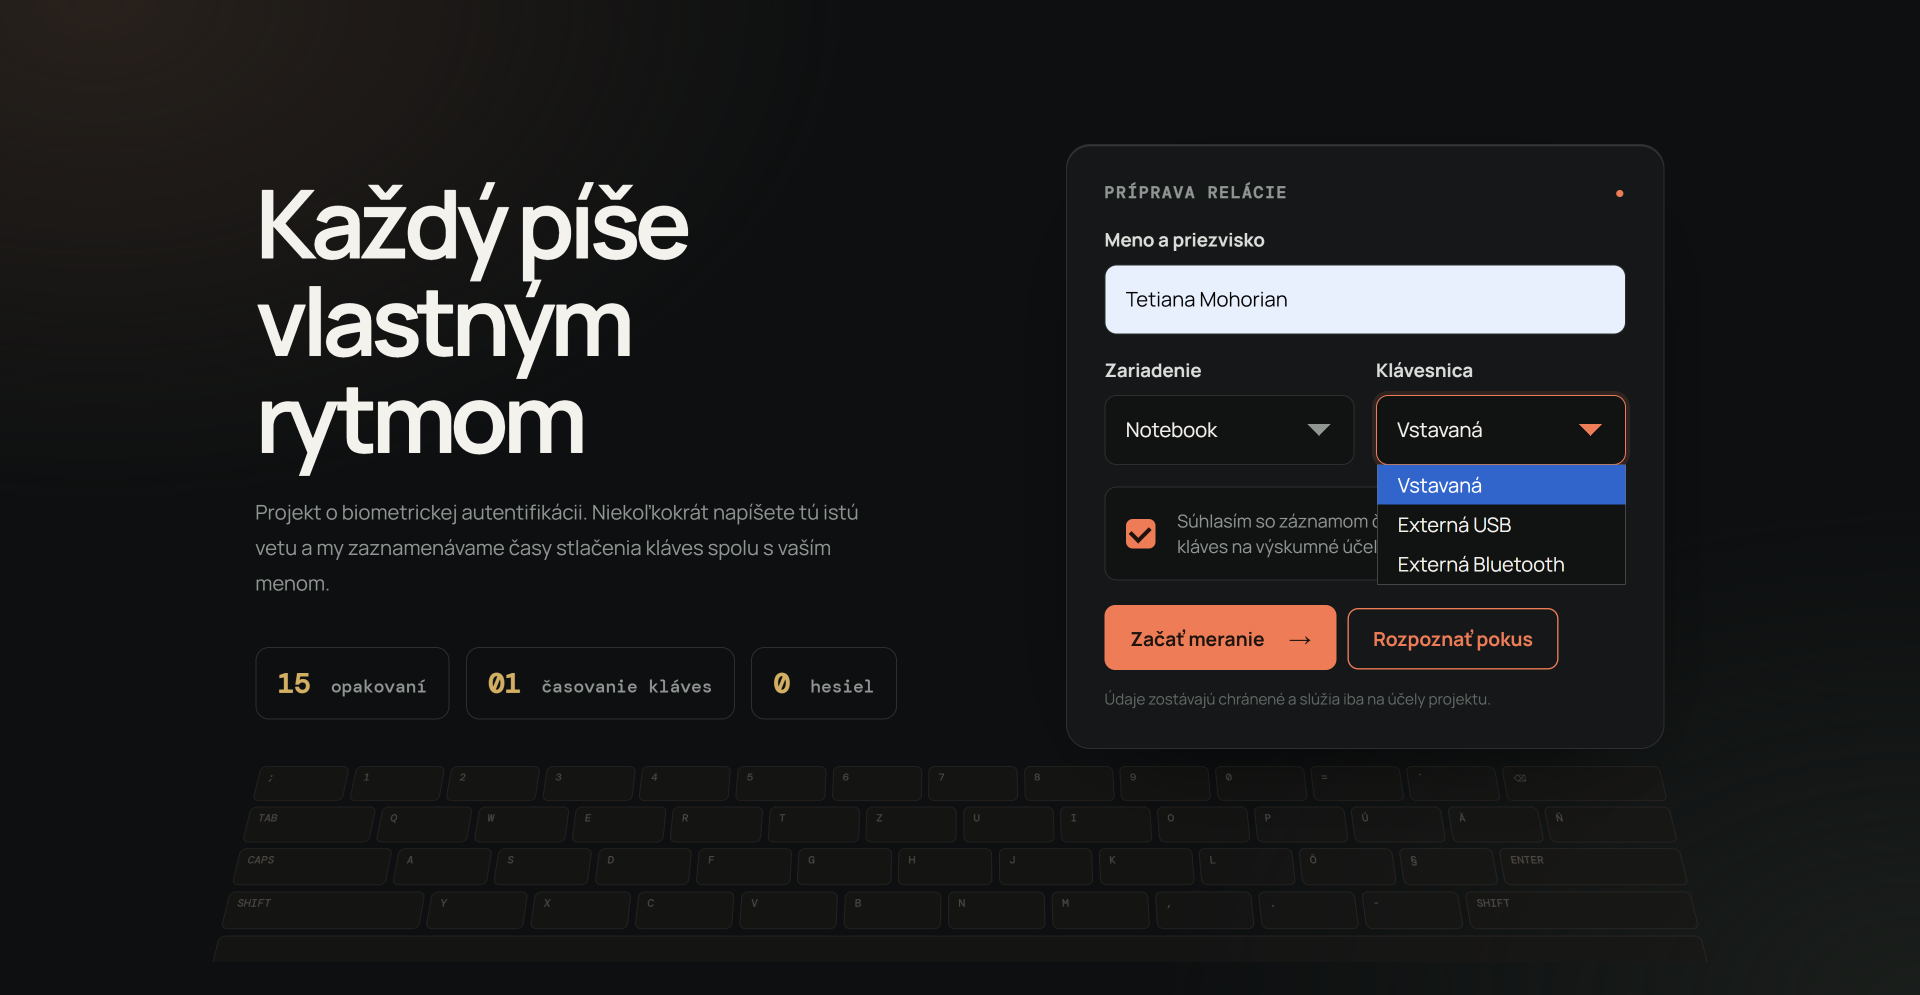
\includegraphics[width=\textwidth]{ui-setup.png}
  \caption{Obrazovka prípravy relácie.}
  \label{fig:setup}
\end{figure}

% Obrázok (obrázok zo súboru figures/ui-run.png): Obrazovka merania: veta, vstupné pole a graf rytmu.
\begin{figure}[ht]
  \centering
  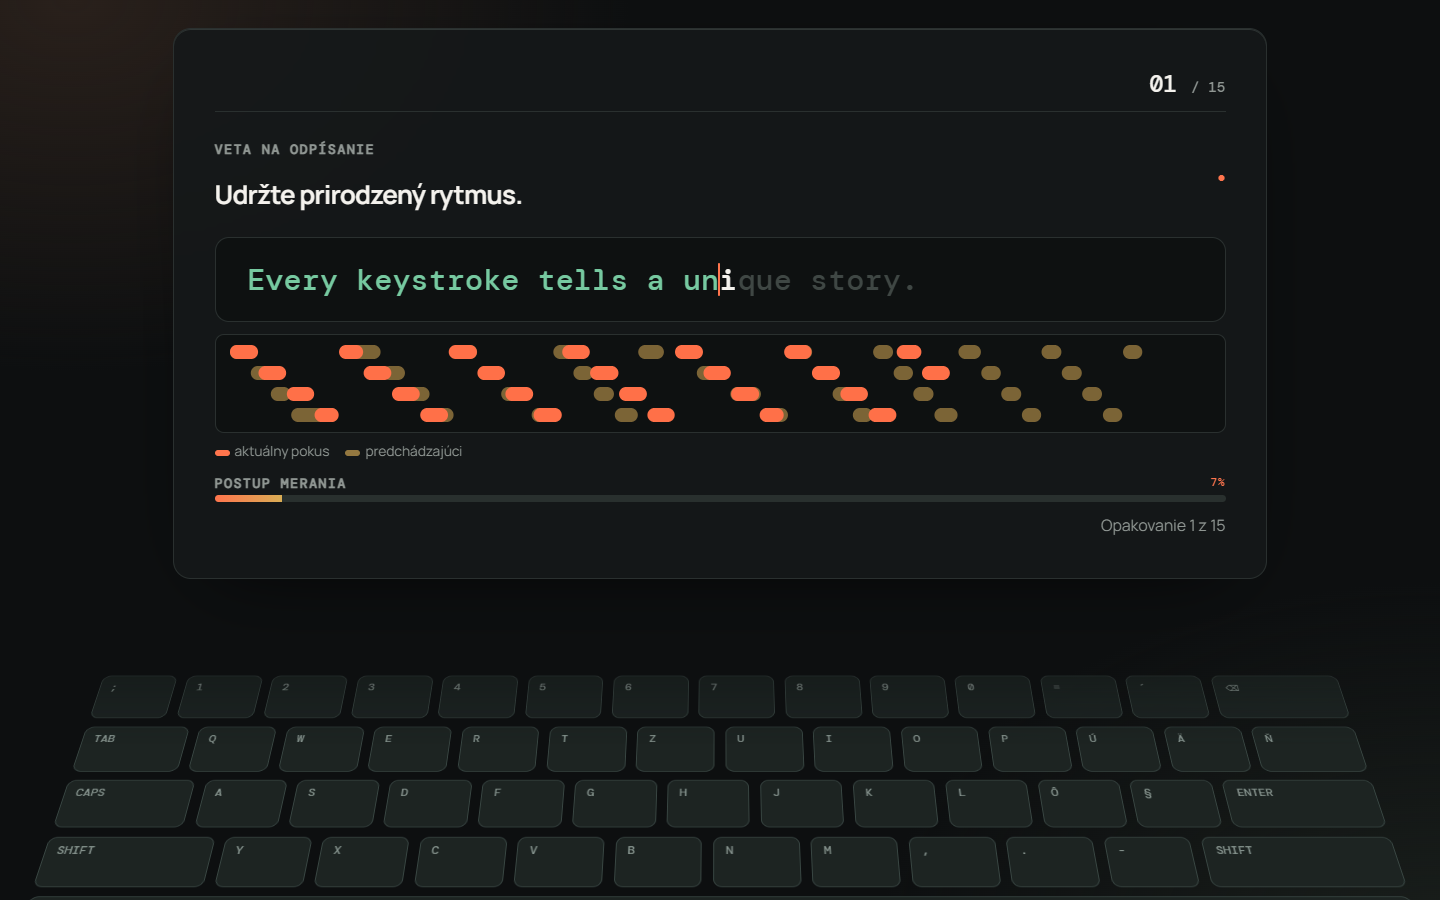
\includegraphics[width=\textwidth]{ui-run.png}
  \caption{Obrazovka merania: veta, vstupné pole a graf rytmu.}
  \label{fig:run}
\end{figure}

% ----- Serverová časť -----
\subsection{Serverová časť}

Server (\code{backend/main.py}) poskytuje rozhranie REST uvedené v
Tab.~\ref{tab:api}. Dokumentácia vo formáte OpenAPI je dostupná na
adrese \code{/docs}.

% Tabuľka: Koncové body API.
\begin{table}[ht]
  \centering
  \small
  \caption{Koncové body API.}
  \label{tab:api}
  \begin{tabularx}{\textwidth}{|l|l|Y|}
    \hline
    \rowcolor[gray]{0.9} \textbf{Metóda} & \textbf{Cesta} & \textbf{Popis} \\
    \hline
    GET  & \code{/api/health} & kontrola dostupnosti \\
    \hline
    POST & \code{/api/sessions} & uloženie dokončenej relácie \\
    \hline
    GET  & \code{/api/sessions} & zoznam relácií bez udalostí (\code{limit}, \code{offset}) \\
    \hline
    GET  & \code{/api/sessions/\{id\}} & metadáta a všetky udalosti jednej relácie \\
    \hline
    GET  & \code{/api/stats} & počet relácií a udalostí \\
    \hline
    POST & \code{/api/identify} & identifikácia jedného pokusu (\code{rows}, \code{mode}) \\
    \hline
    GET  & \code{/api/evaluation} & vyhodnotenie na pokusoch 11--15 (voliteľný parameter \code{mode}) \\
    \hline
    GET  & \code{/api/compare} & porovnanie režimov veta a slovo \\
    \hline
  \end{tabularx}
\end{table}

Relácie sa ukladajú do tabuľky \code{sessions} so stĺpcami \code{id},
\code{participant\_id}, \code{session\_id}, \code{meta\_json},
\code{rows\_json} a \code{created\_at}. Udalosti celej relácie sú uložené
ako jeden JSON dokument. Uloženie je idempotentné: ak už existuje relácia
s rovnakým \code{session\_id}, server nič nezapíše a vráti stav
\code{already\_saved}. Pri chýbajúcom \code{participant\_id},
\code{session\_id}, prázdnom zozname udalostí alebo neznámom režime vráti
chybu 422. Počet kláves v pokuse určuje slovník \code{MODE\_KEYS}
(\code{phrase}: 37, \code{word}: 10), takže validácia a príznaky sa riadia
režimom; relácie bez poľa \code{mode} sa čítajú ako \code{phrase}.

Po každom novo uloženom zázname server na pozadí (\code{BackgroundTasks})
prekreslí súbor \code{accuracy\_chart.png} knižnicou matplotlib: stĺpcový graf
top-1 a top-3 pre vetu a slovo, vypočítaný rovnako ako \code{/api/compare}.
Odpoveď na uloženie sa tým nespomalí a zlyhanie kreslenia uloženie neovplyvní.

% ----- Známe obmedzenia implementácie -----
\subsection{Známe obmedzenia implementácie}
\label{sec:obmedzenia}

Pri interpretácii výsledkov treba zohľadniť tieto obmedzenia:
\begin{itemize}
  \item Pokusy s opravou klávesom Backspace alebo Delete server pri tvorbe
        šablón ignoruje (majú viac ako $n$ stlačení). Klient takéto pokusy
        už nepripustí, no v skorších reláciách sa ešte nachádzajú.
  \item Zariadenie a typ klávesnice sa ukladajú len ako metaúdaje a do
        výpočtov nevstupujú.
  \item Šablóny sa pri každej požiadavke na identifikáciu alebo vyhodnotenie
        počítajú nanovo zo všetkých relácií daného režimu. Pre malý počet
        účastníkov to stačí, pri väčšom objeme dát by bolo vhodné šablóny
        ukladať.
  \item Pri troch a menej účastníkoch je metrika top-3 triviálne rovná
        100\,\%, keďže zoznam obsahuje všetkých účastníkov.
  \item Identifikátorom účastníka je zadané meno, takže databáza obsahuje
        osobné údaje a nemá sa verzionovať ani zverejňovať.
  \item Závislosti klienta sú v \code{package.json} uvedené ako
        \code{latest}; reprodukovateľnosť zaisťuje súbor
        \code{package-lock.json}, v \code{requirements.txt} sú uvedené
        len dolné hranice verzií.
\end{itemize}

% ----- Ukážky kľúčového kódu -----
\subsection{Ukážky kľúčového kódu}

Výpočet vektora príznakov z jedného pokusu (\code{backend/main.py}, skrátené):

\begin{lstlisting}[language=Python]
# 1. Udalosti pokusu zoradíme a rozdelíme na stlačenia a uvoľnenia
frame = pd.DataFrame(rows).sort_values("seq")
downs = frame[frame["event"] == "down"]
ups = frame[frame["event"] == "up"]

# 2. Platný pokus má presne key_count stlačení a uvoľnení
#    (key_count = MODE_KEYS[mode]: 37 pre vetu, 10 pre slovo)
if len(downs) != key_count or len(ups) != key_count:
    raise ValueError(f"an attempt must contain exactly {key_count} key presses and releases")
...

# 3. Doba držania = čas uvoľnenia mínus čas stlačenia tej istej klávesy
holds = []
for _, down in downs.iterrows():
    matching = ups[(ups["code"] == down["code"]) & (ups["seq"] > down["seq"])]
    holds.append(float(matching.iloc[0]["t_ms"]) - float(down["t_ms"]))

# 4. Interval = rozdiel časov dvoch po sebe idúcich stlačení
intervals = [down_times[i] - down_times[i - 1] for i in range(1, len(down_times))]

# 5. Vektor príznakov: n dôb držania + (n-1) intervalov (veta: 73, slovo: 19)
return holds + intervals
\end{lstlisting}

Šablóna účastníka a vzdialenosť nového pokusu od nej:

\begin{lstlisting}[language=Python]
# Každý riadok matice je jeden platný pokus (2n-1 príznakov), pokusy 1-10 jedného režimu
matrix = pd.DataFrame(vectors)

# Šablóna účastníka: priemer a smerodajná odchýlka každého príznaku
mean = matrix.mean().tolist()
std = matrix.std(ddof=0).replace(0, 1).tolist()   # nulová odchýlka -> 1
...

# Vzdialenosť nového pokusu od šablóny (štandardizovaná euklidovská)
distance = sqrt(sum(((v - c) / s) ** 2 for v, c, s in zip(vector, mean, std)))
...

# Neznámy pokus: priemerná odchýlka na jeden príznak je väčšia ako 3
unknown = best_distance / sqrt(len(vector)) > 3
\end{lstlisting}
     % 4 Implementácia
\section{Testovanie a vyhodnotenie}
\label{sec:test}

% ----- Funkčné testovanie klienta -----
\subsection{Funkčné testovanie klienta}

Klientska aplikácia sa overila automatizovaným testom v prehliadači Microsoft
Edge (skript s knižnicou Playwright, ktorý ovládal skutočnú aplikáciu
spustenú vývojovým serverom). Volania API sa v tomto teste nahradili
pripravenými odpoveďami, takže test overuje klienta, nie server.
Výsledky sú v Tab.~\ref{tab:func}.

% Tabuľka: Výsledky funkčného testu klienta.
\begin{table}[!htbp]
  \centering
  \small
  \caption{Výsledky funkčného testu klienta.}
  \label{tab:func}
  \begin{tabularx}{\textwidth}{|Y|M{2.4cm}|}
    \hline
    \rowcolor[gray]{0.9} \textbf{Kontrolovaná vlastnosť} & \textbf{Výsledok} \\
    \hline
    Tlačidlo „Začať meranie“ je neaktívne bez mena a súhlasu & splnené \\
    \hline
    Vstupné pole je po prechode na meranie aktívne (fokus) & splnené \\
    \hline
    Nesprávny text sa zamietne, pole sa vyprázdni a zobrazí sa chyba & splnené \\
    \hline
    Správny pokus sa započíta a zvýši počítadlo & splnené \\
    \hline
    Po 15 pokusoch sa zobrazí súhrn (15 pokusov) & splnené \\
    \hline
    Odoslaná relácia obsahuje $15 \times 74 = 1110$ udalostí & splnené \\
    \hline
    Odoslanie vráti potvrdenie, tlačidlo „Späť“ zachová zadané meno & splnené \\
    \hline
    Režim identifikácie zobrazí výsledok a umožní ho zopakovať & splnené \\
    \hline
    Chyby v konzole prehliadača & žiadne \\
    \hline
  \end{tabularx}
\end{table}

Počet udalostí vyplýva z toho, že jeden pokus s vetou má 37 stlačení a 37
uvoľnení, teda 74 udalostí (pri slove je to 20).

Tento test sa vykonal pred zavedením režimu slova. Neskoršie zmeny
(automatické uloženie relácie, okamžité zrušenie pokusu pri Backspace alebo
nesprávnom znaku, výber režimu) sa overili
prekladom klienta, ručným vyskúšaním režimu slova a simuláciou komponentu
merania v prostredí jsdom (nesprávny znak vyprázdni pole a zobrazí
hlásenie); automatizovaný test v prehliadači sa po týchto zmenách
neopakoval.

% ----- Vyhodnotenie identifikácie -----
\subsection{Vyhodnotenie identifikácie}

Metóda identifikácie sa vyhodnocuje podľa protokolu z podkapitoly~\ref{sec:protokol}:
šablóny z pokusov 1--10, testovanie na pokusoch 11--15. Vyhodnotenie
vracia koncový bod \code{/api/evaluation}.

\paragraph{Zozbierané dáta.}
Údaje o súbore dát (stav databázy k 20.~11.~2026) sú v Tab.~\ref{tab:data}. Mená účastníkov sú v tejto
práci nahradené označeniami Účastník 1 až 5 (traja z účastníkov sú autormi práce;
číslovanie je náhodné).

% Tabuľka: Charakteristika zozbieraných dát.
\begin{table}[!htbp]
  \centering
  \small
  \caption{Charakteristika zozbieraných dát.}
  \label{tab:data}
  \begin{tabularx}{\textwidth}{|Y|M{6cm}|}
    \hline
    \rowcolor[gray]{0.9} \textbf{Ukazovateľ} & \textbf{Hodnota} \\
    \hline
    Počet účastníkov & 5 \\
    \hline
    Počet relácií & 14 (9 s vetou, 5 so slovom) \\
    \hline
    Počet zaznamenaných klávesových udalostí & 11\,560 \\
    \hline
    Počet testovacích pokusov (11--15) vo vyhodnotení (veta) & 38 \\
    \hline
    Zloženie podľa zariadenia (notebook / stolný počítač) & notebook: 14 relácií, stolný počítač: 0 \\
    \hline
    Zloženie podľa klávesnice (vstavaná / USB / Bluetooth) & vstavaná: 7 relácií, externá USB: 7 relácií, Bluetooth: 0 \\
    \hline
  \end{tabularx}
\end{table}

Počty relácií a udalostí pochádzajú z koncového bodu \code{/api/stats} a zahŕňajú aj päť relácií s režimom slova (tri od
Účastníka~1 na externej USB klávesnici a po jednej od Účastníka~3
a Účastníka~5 so vstavanou klávesnicou). Vyhodnotenie
identifikácie v tejto podkapitole sa týka režimu vety, teda deviatich relácií.
Všetky relácie sa zaznamenali na notebooku. Vo vete sú štyri relácie
s externou USB klávesnicou (tri relácie Účastníka~5 a jedna relácia Účastníka~2)
a päť so vstavanou klávesnicou; vplyv zariadenia sa preto nedá vyhodnotiť
a vplyv klávesnice len veľmi obmedzene.
V režime vety majú štyria účastníci po jednej relácii, Účastník~5 má relácií päť.
Z nich je jedna celá neplatná (38 až 39 stlačení namiesto 37 v každom pokuse)
a v ďalšej je neplatný jeden pokus (tretí, v časti určenej na šablónu). Pri
Účastníkovi~1 sú dva testovacie pokusy neplatné (39 stlačení namiesto 37,
čo zodpovedá jednému preklepu a jeho oprave klávesom Backspace). Neplatné
pokusy sa pri tvorbe šablón aj vo vyhodnotení ignorujú
(podkapitola~\ref{sec:priznaky}).

\paragraph{Úspešnosť.}
Výsledky z koncového bodu \code{/api/evaluation} sú v Tab.~\ref{tab:vysledky}.

% Tabuľka: Úspešnosť identifikácie na testovacích pokusoch 11--15.
\begin{table}[!htbp]
  \centering
  \small
  \caption{Úspešnosť identifikácie (pokusy 11--15)}
  \label{tab:vysledky}
  \begin{tabularx}{\textwidth}{|Y|M{3.5cm}|}
    \hline
    \rowcolor[gray]{0.9} \textbf{Metrika} & \textbf{Hodnota} \\
    \hline
    Počet testovacích pokusov (\code{total}) & 38 \\
    \hline
    Správne na prvom mieste & 30 \\
    \hline
    Top-1 (\code{top1}) & 78,95\,\% \\
    \hline
    Správny účastník medzi prvými tromi & 37 \\
    \hline
    Top-3 (\code{top3}) & 97,37\,\% \\
    \hline
  \end{tabularx}
\end{table}

Úspešnosť podľa účastníka uvádza Tab.~\ref{tab:participant} a maticu zámen
Tab.~\ref{tab:confusion} (v riadkoch je skutočný účastník, v stĺpcoch predikcia). Pokus
označený ako neznámy sa počíta ako chybný.

% Tabuľka: Úspešnosť top-1 podľa účastníka.
\begin{table}[!htbp]
  \centering
  \small
  \caption{Úspešnosť top-1 podľa účastníka.}
  \label{tab:participant}
  \begin{tabularx}{\textwidth}{|Y|C|C|C|}
    \hline
    \rowcolor[gray]{0.9} \textbf{Účastník} & \textbf{Testovacích pokusov} & \textbf{Správne} & \textbf{Top-1} \\
    \hline
    Účastník 1 & 3 & 2 & 66,7\,\% \\
    \hline
    Účastník 2 & 5 & 4 & 80,0\,\% \\
    \hline
    Účastník 3 & 5 & 5 & 100,0\,\% \\
    \hline
    Účastník 4 & 5 & 2 & 40,0\,\% \\
    \hline
    Účastník 5 & 20 & 17 & 85,0\,\% \\
    \hline
    Spolu & 38 & 30 & 78,9\,\% \\
    \hline
  \end{tabularx}
\end{table}

% Tabuľka: Matica zámen (riadky: skutočný účastník, stĺpce: predikcia).
\begin{table}[!htbp]
  \centering
  \small
  \caption{Matica zámen}
  \label{tab:confusion}
  \begin{tabularx}{\textwidth}{|Y|C|C|C|C|C|C|}
    \hline
    \rowcolor[gray]{0.9}  & \textbf{Úč.~1} & \textbf{Úč.~2} & \textbf{Úč.~3} & \textbf{Úč.~4} & \textbf{Úč.~5} & \textbf{neznámy} \\
    \hline
    Účastník 1 & 2 & 1 & 0 & 0 & 0 & 0 \\
    \hline
    Účastník 2 & 0 & 4 & 0 & 0 & 0 & 1 \\
    \hline
    Účastník 3 & 0 & 0 & 5 & 0 & 0 & 0 \\
    \hline
    Účastník 4 & 0 & 0 & 3 & 2 & 0 & 0 \\
    \hline
    Účastník 5 & 0 & 0 & 3 & 0 & 17 & 0 \\
    \hline
  \end{tabularx}
\end{table}

Platia tu aj obmedzenia z podkapitoly~\ref{sec:obmedzenia}. Vzorka je malá (38 pokusov), takže jeden
pokus mení top-1 približne o 3 percentuálne body. Počet pokusov na účastníka
je nerovnaký: Účastník~5 prispieva 20 z 38 pokusov, takže celkové čísla sú
ním výrazne ovplyvnené. Pri piatich účastníkoch so šablónou by náhodný
odhad dosiahol top-1 20\,\% a top-3 60\,\%.

\paragraph{Postup na získanie čísel.} Po zbere dát spustite server a
otvorte v prehliadači adresu \code{/api/evaluation} servera; odpoveď
obsahuje polia \code{top1}, \code{top3}, \code{total} a \code{confusion}.
Údaje o súbore dát poskytujú \code{/api/stats} a \code{/api/sessions}.

% ----- Príklad identifikácie jedného pokusu -----
\subsection{Príklad identifikácie jedného pokusu}
\label{sec:priklad-real}

Postup z podkapitoly~\ref{sec:priklad} je ďalej ukázaný na jednom skutočnom
testovacom pokuse (15. pokus tretej relácie Účastníka~5, teda pokus mimo
šablóny). Pokus bol vybraný ako ilustračný, nie ako typický: ide o jeden
z pokusov, pri ktorých sa v prvej trojke objavili práve traja účastníci,
ktorí sú autormi práce. Čísla v Tab.~\ref{tab:priklad-real} vrátila funkcia
identifikácie servera. Pokus mal 37 stlačení, vektor $m=73$ príznakov a celkový
čas písania približne 7,2\,s.

% Tabuľka: Skutočný výsledok identifikácie jedného testovacieho pokusu.
\begin{table}[!htbp]
  \centering
  \small
  \caption{Identifikácia jedného testovacieho pokusu}
  \label{tab:priklad-real}
  \begin{tabularx}{\textwidth}{|Y|C|C|C|}
    \hline
    \rowcolor[gray]{0.9} \textbf{Poradie a účastník} & \textbf{Vzdialenosť $d_i$} & \textbf{Váha $w_i=1/d_i$} & \textbf{Miera podobnosti $p_i$} \\
    \hline
    1. Účastník 5 & 4,955 & 0,2018 & 64,6\,\% \\
    \hline
    2. Účastník 3 & 16,535 & 0,0605 & 19,4\,\% \\
    \hline
    3. Účastník 1 & 20,016 & 0,0500 & 16,0\,\% \\
    \hline
  \end{tabularx}
\end{table}

Skutočný autor pokusu je na prvom mieste. Kontrola neznámeho pokusu podľa
vzorca~\eqref{eq:unknown} dáva $d_{\min}/\sqrt{m} = 4{,}955/\sqrt{73} \approx 0{,}58$,
čo je výrazne menej ako prah 3, takže pokus sa neoznačí ako neznámy. Rozdiel
vzdialeností medzi prvým a druhým účastníkom je výrazný (5,0 oproti 16,5);
64,6\,\% je len relatívny podiel medzi tromi najbližšími šablónami
(vzorec~\eqref{eq:share}).

% ----- Diskusia -----
\subsection{Diskusia}

Z Tab.~\ref{tab:confusion} vyplývajú tieto pozorovania. Osem z 38 pokusov
bolo určených nesprávne: tri pokusy Účastníka~4 a tri pokusy Účastníka~5 boli
priradené Účastníkovi~3, jeden pokus Účastníka~1 bol priradený Účastníkovi~2
a jeden pokus Účastníka~2 bol označený ako neznámy. Šesť z ôsmich chýb
teda smeruje k Účastníkovi~3, ktorý bol sám rozpoznaný vo všetkých piatich
pokusoch. V jednom prípade z 38 nebol správny účastník ani medzi prvými
tromi (top-3 je 37 z 38).

Účastník~5 dosiahol 85,0\,\% (17 z 20) na pokusoch zo štyroch platných relácií.
Najslabšie je rozpoznaný Účastník~4 (40\,\%), ktorého
pokusy sa najčastejšie zamieňajú s Účastníkom~3.

% ----- Príčiny zámen -----
\paragraph{Príčina zámen.}
Zámeny smerujúce k Účastníkovi~3 sa dajú vysvetliť šírkou jeho šablóny.
Štandardizovaná vzdialenosť (vzorec~\eqref{eq:dist}) delí odchýlku od
priemeru smerodajnou odchýlkou šablóny, takže široká šablóna zmenšuje
vzdialenosť aj pre pokusy iných účastníkov a priťahuje ich k sebe. Údaje
v Tab.~\ref{tab:sigma} to podporujú: šablóna Účastníka~3 má najväčšiu
priemernú smerodajnú odchýlku príznakov (145,7\,ms, u Účastníkov~1 a~5 len
51,0 a 53,5\,ms) a cudzie pokusy sú k nej v priemere najbližšie
($d/\sqrt{m} = 2{,}32$ oproti 3,39 až 6,76 pri ostatných šablónach).
Účastník~3 píše aj najpomalšie (pokus mu trvá približne 21\,s, ostatným 8 až 15\,s).
Účastník~2 má tiež širokú šablónu (140,4\,ms), no priťahuje len jednu zámenu,
takže šírka šablóny nie je jediný činiteľ.

% Tabuľka: Šírka šablón a vzdialenosť cudzích pokusov.
\begin{table}[!htbp]
  \centering
  \small
  \caption{Šírka šablón a vzdialenosť cudzích pokusov}
  \label{tab:sigma}
  \begin{tabularx}{\textwidth}{|Y|C|C|C|}
    \hline
    \rowcolor[gray]{0.9} \textbf{Účastník} & \textbf{Priem. smerodajná odchýlka šablóny [ms]} & \textbf{Priem. čas pokusu [s]} & \textbf{Priem. $d/\sqrt{m}$ cudzích pokusov} \\
    \hline
    Účastník 1 & 51,0 & 8,7 & 4,35 \\
    \hline
    Účastník 2 & 140,4 & 15,1 & 3,39 \\
    \hline
    Účastník 3 & 145,7 & 21,2 & 2,32 \\
    \hline
    Účastník 4 & 63,6 & 12,8 & 6,76 \\
    \hline
    Účastník 5 & 53,5 & 7,9 & 6,67 \\
    \hline
  \end{tabularx}
\end{table}

Domnienku sme overili aj jednoduchým pokusom: namiesto smerodajnej odchýlky
každej šablóny sme pre všetkých účastníkov použili spoločnú odchýlku (priemer
odchýlok všetkých šablón, teda bez údajov z testovacích pokusov). Top-1 vtedy
vzrástol z 31 na 37 z 38 pokusov (97,4\,\%) a top-3 na 38 z 38; zostala jediná
chyba (pokus Účastníka~5 priradený Účastníkovi~4) a žiadna už nesmeruje
k Účastníkovi~3. Porovnanie je bez pravidla pre neznámy pokus, preto je
základ 31 z 38 a nie 30 z 38. Ide o jeden pokus na malej vzorke, nie o hotové
vylepšenie metódy; do implementácie sa nezaviedol.

% ----- Obmedzenia vyhodnotenia -----
Vplyv zariadenia sa nedá posúdiť, pretože všetky relácie vznikli na
notebooku; vplyv klávesnice sa nedá oddeliť od vplyvu osoby (tri zo štyroch
relácií vety s externou USB klávesnicou patria jednému účastníkovi). Šablóna sa
počíta z desiatich pokusov s 73 príznakmi, takže odhad smerodajnej odchýlky
je nepresný. Pri troch až piatich testovacích pokusoch na osobu (Účastník~5 ich
má 20) mení jeden pokus úspešnosť účastníka o 20 až 33 percentuálnych bodov,
preto rozdiely medzi účastníkmi (od 40\,\% do 100\,\%) treba vnímať opatrne.
Účastník~1 má navyše len tri testovacie pokusy, pretože dva boli neplatné pre
opravu klávesom Backspace. Jediný pokus označený ako neznámy patrí účastníkovi,
ktorý bol inak správne rozpoznaný; prah~3 pri identifikácii by sa preto mal kalibrovať
podobne ako prah v analýze overenia (podkapitola~\ref{sec:kalibracia}).

% ----- Chyby overenia a kalibrácia prahu -----
\subsection{Chyby overenia a kalibrácia prahu}
\label{sec:kalibracia}

Analýza z podkapitoly~\ref{sec:overenie} sa vykonala skriptom
\code{backend/far\_frr.py} na rovnakých dátach ako identifikácia v režime vety
(5 účastníkov, 38 testovacích pokusov, stav databázy k 20.~11.~2026).
Tab.~\ref{tab:kalibracia} uvádza počty porovnaní a vybraný prah,
Tab.~\ref{tab:chyby-overenia} chyby na pokusoch 14--15, ktoré sa pri výbere prahu
nepoužili. Obr.~\ref{fig:farfrr} ukazuje krivky FAR a FRR podľa prahu
a Obr.~\ref{fig:skore} rozdelenie skóre vlastných a cudzích porovnaní. Na
Obr.~\ref{fig:farfrr} je zelená čiara kalibrovaný prah a prerušovaná čiara pôvodný
prah 3; na Obr.~\ref{fig:skore} sú hodnoty nad 8 započítané do posledného stĺpca.

% Tabuľka: Kalibrácia prahu overenia (režim vety).
\begin{table}[!htbp]
  \centering
  \small
  \caption{Kalibrácia prahu overenia (režim vety).}
  \label{tab:kalibracia}
  \begin{tabularx}{\textwidth}{|Y|M{3.5cm}|}
    \hline
    \rowcolor[gray]{0.9} \textbf{Ukazovateľ} & \textbf{Hodnota} \\
    \hline
    Kalibračné porovnania (pokusy 11--13), vlastné & 22 \\
    \hline
    Kalibračné porovnania (pokusy 11--13), cudzie & 88 \\
    \hline
    Kalibrovaný prah $\tau^{*}$ & 2,13 \\
    \hline
    EER na kalibračných pokusoch & 13,6\,\% \\
    \hline
    Testovacie porovnania (pokusy 14--15), vlastné / cudzie & 16 / 64 \\
    \hline
  \end{tabularx}
\end{table}

% Tabuľka: Chyby overenia na nezávislých pokusoch 14--15 pri pôvodnom a kalibrovanom prahu.
\begin{table}[!htbp]
  \centering
  \small
  \caption{Chyby overenia na pokusoch 14--15}
  \label{tab:chyby-overenia}
  \begin{tabularx}{\textwidth}{|Y|C|C|}
    \hline
    \rowcolor[gray]{0.9} \textbf{Prah} & \textbf{FAR} & \textbf{FRR} \\
    \hline
    pôvodný, $\tau = 3$ & 35,9\,\% & 12,5\,\% \\
    \hline
    kalibrovaný, $\tau^{*} = 2{,}13$ & 10,9\,\% & 18,8\,\% \\
    \hline
  \end{tabularx}
\end{table}

% Obrázok (graf z backend/far_frr.py): krivky FAR a FRR.
\begin{figure}[H]
  \centering
  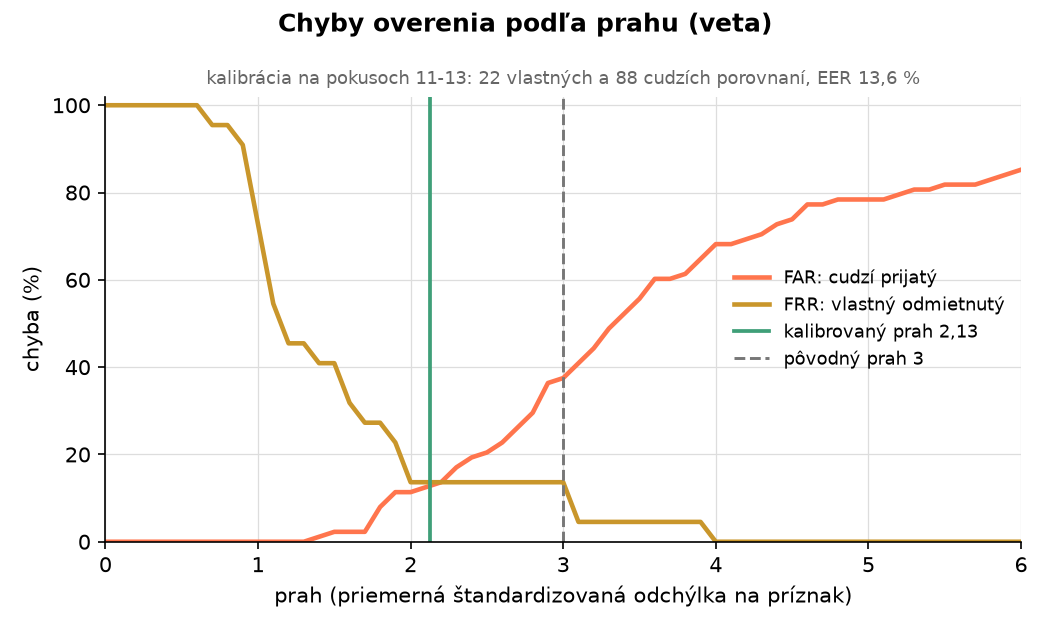
\includegraphics[width=\textwidth]{far_frr_phrase.png}
  \caption{Krivky FAR a FRR podľa prahu}
  \label{fig:farfrr}
\end{figure}

% Obrázok (graf z backend/far_frr.py): rozdelenie skóre.
\begin{figure}[H]
  \centering
  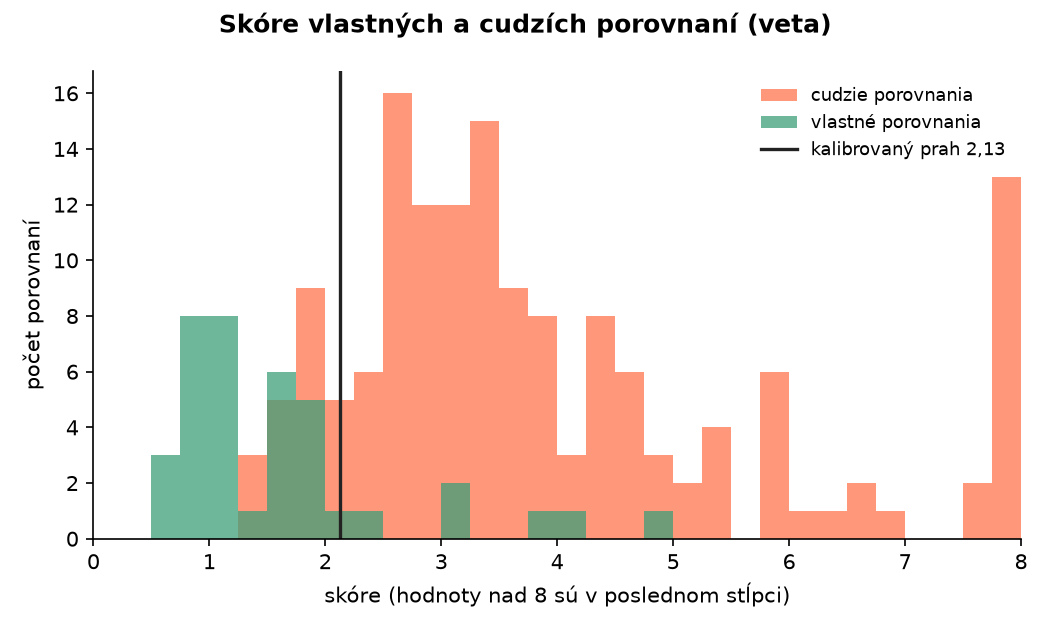
\includegraphics[width=\textwidth]{score_distribution_phrase.png}
  \caption{Rozdelenie skóre vlastných a cudzích porovnaní}
  \label{fig:skore}
\end{figure}

Starý prah 3 je pre overenie príliš voľný: prepustil by viac ako tretinu
cudzích pokusov (35,9\,\%). Nový prah 2,13 túto chybu zníži na 10,9\,\% (7 zo 64
cudzích porovnaní), ale systém potom častejšie odmietne aj vlastný pokus
(18,8\,\% namiesto 12,5\,\%, teda 3 zo 16 pokusov). Čo je lepšie, závisí od
použitia: tam, kde treba chrániť prístup, je dôležitejší nízky FAR. Priemer oboch
chýb na pokusoch 14--15 vyšiel 14,9\,\%, podobne ako EER 13,6\,\% z kalibrácie,
takže prah nie je vyladený len na dáta, z ktorých vznikol.

Obr.~\ref{fig:skore} ukazuje, prečo sa chyby nedajú odstrániť úplne. Skóre
vlastných porovnaní sa drží okolo 1 až 2, skóre cudzích je väčšinou nad 2,5
a má dlhý chvost, ale obe rozdelenia sa trochu prekrývajú.

V režime slova (3 účastníci, 25 testovacích pokusov) vyšiel prah 1,93 a EER
1,7\,\%. Na pokusoch 14--15 bolo FAR 0\,\% a FRR 10\,\%, kým prah 3 by dal FAR
30\,\% a FRR 0\,\%. Dát je tu však málo (10 vlastných a 20 cudzích porovnaní)
a veľká časť patrí jednému človeku (15 z 25 pokusov má Účastník~1), takže to
berieme len ako ilustráciu.

Aj čísla pre vetu sú orientačné. Testovacích vlastných porovnaní je len 16, takže
jeden pokus posunie FRR o 6,25 percentuálneho bodu. Rozdelenie na kalibračné
a testovacie pokusy je pevné (podľa poradia pokusu) a bez krížovej validácie.
Čísla aj grafy sa dajú znovu vytvoriť príkazom \code{python far\_frr.py} (alebo
\code{python far\_frr.py {-}{-}mode word}) v priečinku \code{backend}; skript
vypíše výsledky a nakreslí grafy do \code{docs/figures}.

% ----- Porovnanie vety a slova -----
\subsection{Porovnanie vety a slova}
\label{sec:test-porovnanie}

Na porovnanie režimov slúži koncový bod \code{/api/compare}. Pre každý režim sa podľa protokolu z
podkapitoly~\ref{sec:protokol} zobrazí presnosť top-1 a top-3, podiel pokusov
označených ako neznáme, priemerný čas pokusu a počet príznakov (73 pre vetu,
19 pre slovo). Výpočet sa robí len na účastníkoch, ktorí absolvovali oba
režimy (podkapitola~\ref{sec:porovnanie}); ak ich je menej než dvaja,
server vráti všetky dáta s poznámkou, že porovnanie nie je spravodlivé.

Funkčnosť výpočtu sa overila na syntetických dátach troch účastníkov v oboch
režimoch (správne počty príznakov 73 a 19 a rozdielne priemerné časy pokusu)
a na existujúcich dátach (výsledky pre vetu sa po zavedení režimov nezmenili).
Podľa stavu databázy k 20.~11.~2026 má už aj režim slova dáta od troch
účastníkov (Účastník~1, 3 a 5), ktorí písali aj vetu, takže porovnanie
počítame na týchto troch ľuďoch. Výsledky sú v Tab.~\ref{tab:porovnanie} a na Obr.~\ref{fig:porovnanie}.

% Tabuľka: Porovnanie vety a slova na troch spoločných účastníkoch.
\begin{table}[!htbp]
  \centering
  \small
  \caption{Porovnanie vety a slova}
  \label{tab:porovnanie}
  \begin{tabularx}{\textwidth}{|Y|C|C|}
    \hline
    \rowcolor[gray]{0.9} \textbf{Ukazovateľ} & \textbf{Veta} & \textbf{Slovo} \\
    \hline
    Počet príznakov & 73 & 19 \\
    \hline
    Testovacie pokusy (11--15) & 28 & 25 \\
    \hline
    Top-1 & 85,71\,\% & 100,0\,\% \\
    \hline
    Top-3 & 100,0\,\% & 100,0\,\% \\
    \hline
    Podiel pokusov označených ako neznáme & 3,57\,\% & 0,0\,\% \\
    \hline
    Priemerný čas pokusu & 9,6~s & 2,7~s \\
    \hline
  \end{tabularx}
\end{table}

% Obrázok (graf generuje server po každom uložení relácie): presnosť vety a slova.
\begin{figure}[H]
  \centering
  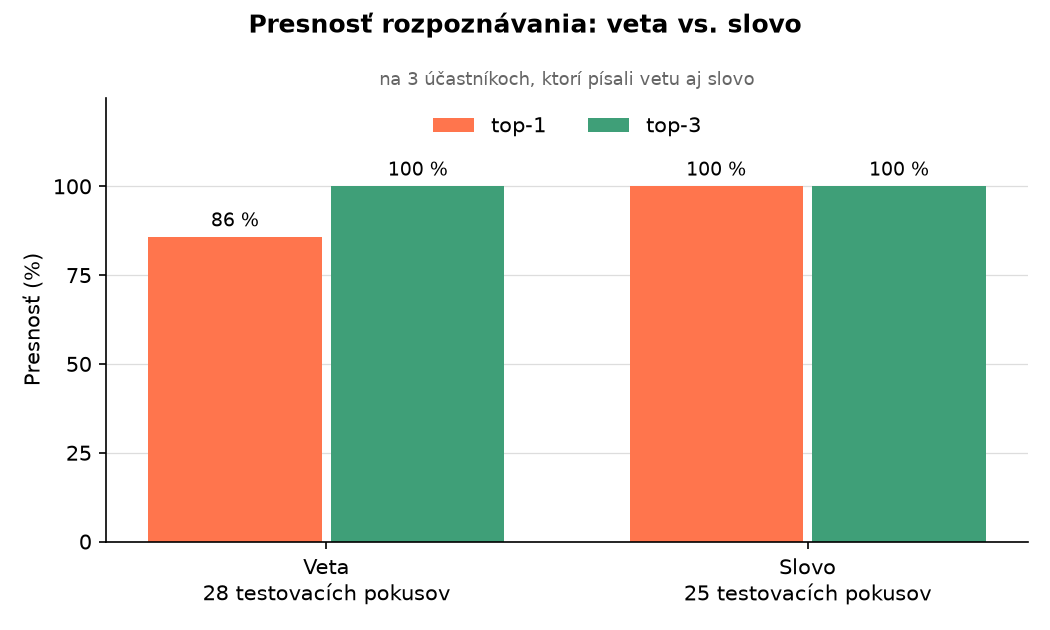
\includegraphics[width=\textwidth]{accuracy_chart.png}
  \caption{Presnosť vety a slova}
  \label{fig:porovnanie}
\end{figure}

Čísla netreba preceňovať. Pri troch šablónach je náhodný odhad pre top-1 33\,\%
a top-3 je vždy 100\,\%, lebo v zozname sú všetci traja účastníci. Pokusy sú
rozdelené nerovnomerne: pri vete je 20 z 28 pokusov od Účastníka~5, pri slove
15 z 25 od Účastníka~1. Šablóna Účastníka~1 pre slovo vznikla zo všetkých troch
jeho relácií, pre vetu má len jednu, takže náskok slova môže byť čiastočne len
dôsledok väčšieho množstva dát. Spoľahlivo vieme povedať iba toľko, že pokus so
slovom trvá asi 3,5-krát kratšie (2,7~s oproti 9,6~s) a že na týchto troch
ľuďoch slovo nedopadlo horšie ako veta.
        % 5 Testovanie a vyhodnotenie
\section{Príručka na používanie riešenia}
\label{sec:prirucka}

Zdrojový kód je archivovaný v repozitári GitHub~\cite{repo}.

% ----- Požiadavky -----
\subsection{Požiadavky}

\begin{itemize}
  \item Node.js a npm (vyvíjané s Node.js 24),
  \item Python 3 (vyvíjané s verziou 3.14),
  \item prehliadač s podporou \code{canvas} a \code{performance.now()}
        (testované v Microsoft Edge).
\end{itemize}

% ----- Inštalácia -----
\subsection{Inštalácia}

\begin{lstlisting}
# 1. Stiahnutie projektu
git clone https://github.com/tetianamohorian23/bsb-keystroke.git
cd bsb-keystroke

# 2. Klient (React)
npm install

# 3. Server (Python) vo vlastnom virtuálnom prostredí
cd backend
python -m venv .venv
.venv\Scripts\activate          # Windows
pip install -r requirements.txt
\end{lstlisting}

% ----- Spustenie -----
\subsection{Spustenie}

Server a klient sa spúšťajú v dvoch samostatných termináloch.

\begin{lstlisting}
# Terminál 1: server na http://127.0.0.1:8000
cd backend
.venv\Scripts\uvicorn main:app --reload

# Terminál 2: klient (adresu vypíše Vite, zvyčajne http://localhost:5173)
npm run dev
\end{lstlisting}

Vývojový server Vite presmeruje požiadavky na cestu \code{/api} na server
na porte 8000 (nastavenie v \code{vite.config.js}). Databáza
\code{backend/sessions.sqlite3} sa vytvorí automaticky pri prvom spustení.
Produkčná zostava klienta sa vytvorí príkazom \code{npm run build}
do priečinka \code{dist/}.

% ----- Postup pre účastníka -----
\subsection{Postup pre účastníka}

Aplikáciu otvorte na počítači alebo notebooku s fyzickou klávesnicou:
na telefóne a tablete sa zobrazí hlásenie „Nie je podporované“.
\begin{enumerate}
  \item Na úvodnej obrazovke zadajte meno a priezvisko, vyberte zariadenie
        a klávesnicu (pri stolovom počítači nie je ponuka „Vstavaná“),
        v poli „Čo budete písať“ zvoľte vetu alebo slovo a zaškrtnite súhlas.
        Tlačidlo „Začať meranie“ sa aktivuje až po vyplnení mena a súhlasu.
  \item Napíšte zobrazený text rovnako, ako bežne píšete, a potvrďte ho
        klávesom Enter. Backspace a Delete nefungujú: ich stlačenie aj
        nesprávny znak pokus nezapočítajú: vstup sa na chvíľu zamkne,
        zobrazený text sa zatrasie a hlásenie vysvetlí, čo sa stalo; potom
        písanie začnete odznova a počítadlo sa nezvýši. Pokus
        s neuvoľnenou klávesou sa nezapočíta.
  \item Po 15 správnych pokusoch sa zobrazí súhrn (počet pokusov, priemerná
        doba držania klávesy a priemerný čas napísania textu).
  \item Relácia sa na server uloží automaticky, tlačidlo na odoslanie nie je
        potrebné. Ak uloženie zlyhá, zobrazia sa tlačidlá „Skúsiť znova“
        a „Stiahnuť CSV“. Opakované odoslanie tej istej relácie sa nezapíše
        znova.
\end{enumerate}

% ----- Identifikácia pokusu -----
\subsection{Identifikácia pokusu}

Na úvodnej obrazovke tlačidlo „Rozpoznať pokus“ otvorí režim, v ktorom
účastník napíše zvolený text (vetu alebo slovo, podľa režimu zvoleného na
úvodnej obrazovke) jedenkrát. Server vráti troch najpodobnejších
účastníkov s relatívnou mierou podobnosti, alebo označí pokus ako neznámy.
Režim vyžaduje, aby v databáze existovali relácie s dostatočným počtom
platných pokusov.

Výsledok identifikácie na skutočných dátach ukazuje Obr.~\ref{fig:identify}: pokus napísal účastník, ktorého šablóna je v databáze, a server ho
priradil správne. Okrem najpodobnejšieho účastníka zobrazí aplikácia aj
ďalších dvoch kandidátov. Percentá udávajú len relatívne poradie medzi
troma najbližšími šablónami, nie pravdepodobnosť zhody.

% Obrázok (obrázok zo súboru figures/ui-identify.png): Identifikácia pokusu na skutočných dátach: najpodobnejší účastník a relatívna miera podobnosti troch najlepších kandidátov.
\begin{figure}[ht]
  \centering
  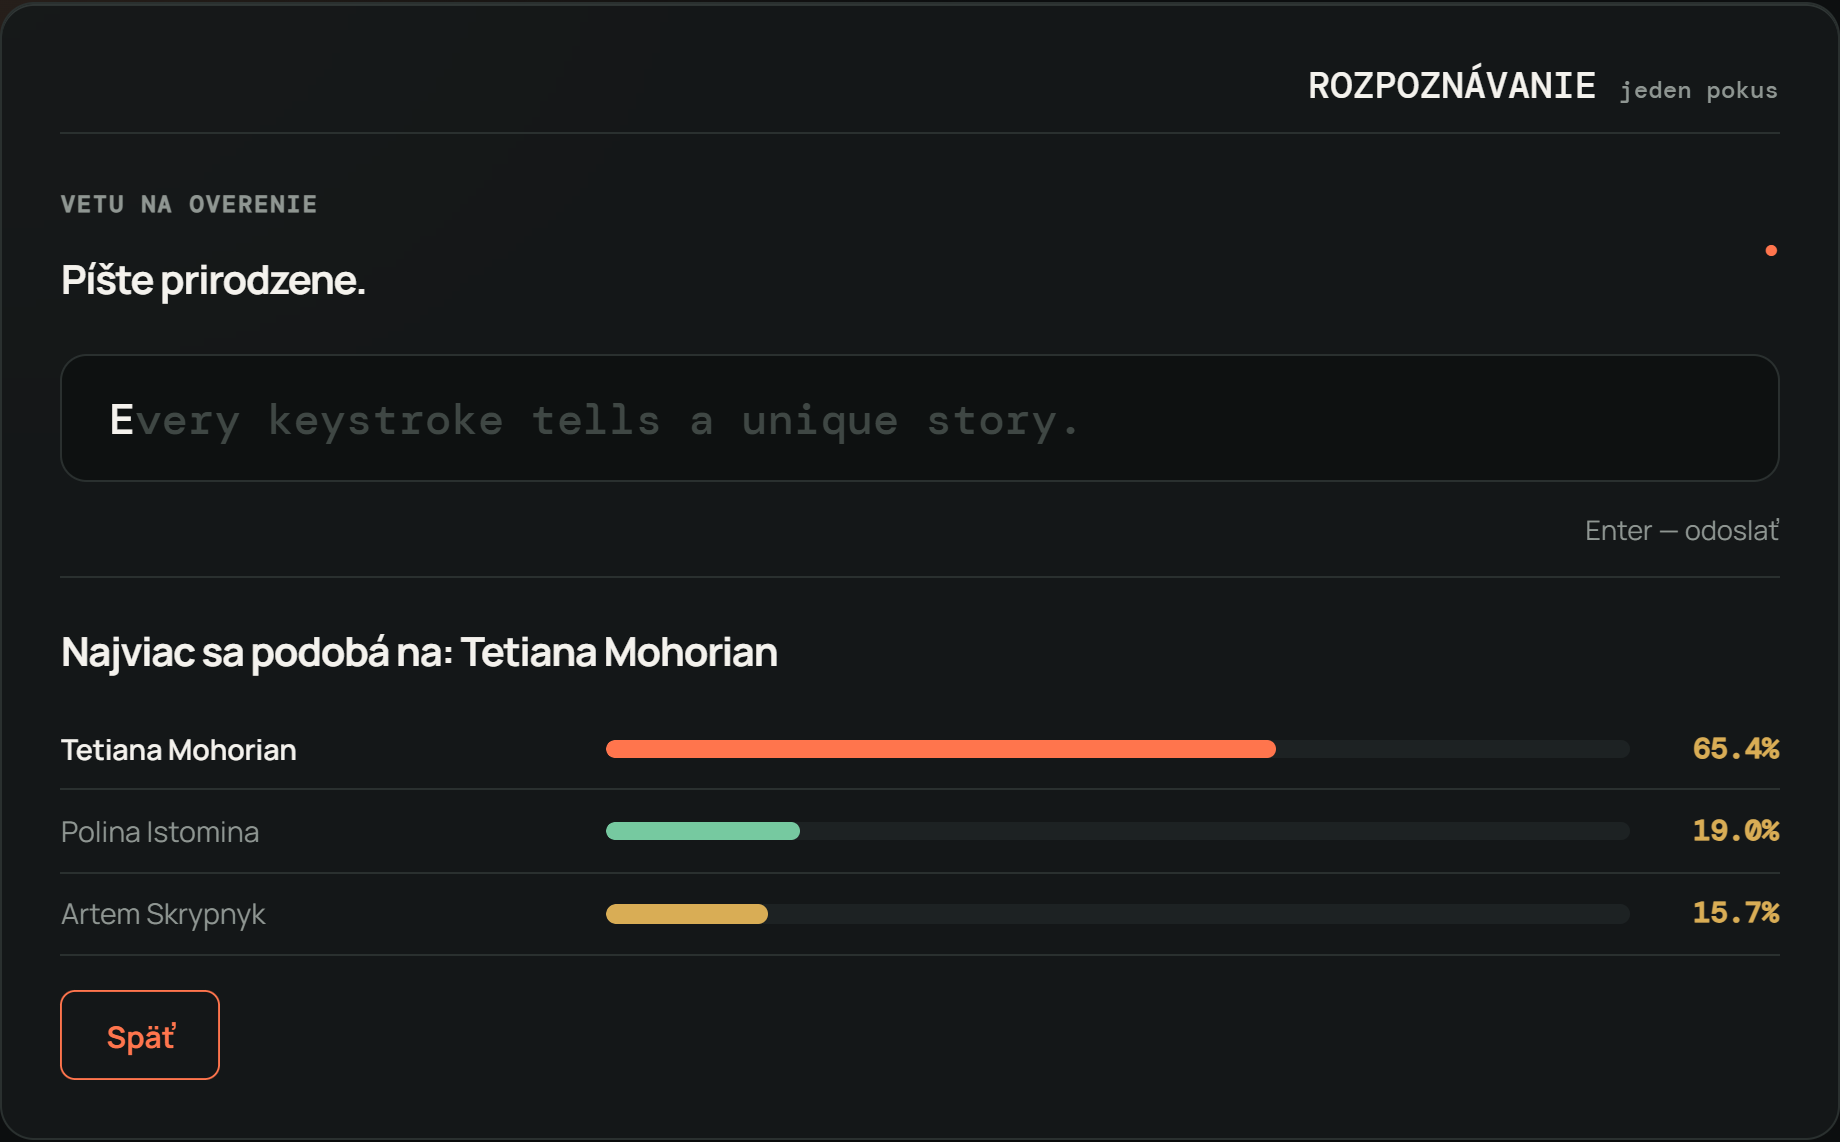
\includegraphics[width=\textwidth]{ui-identify.png}
  \caption{Identifikácia pokusu na skutočných dátach: najpodobnejší účastník
           a relatívna miera podobnosti troch najlepších kandidátov.}
  \label{fig:identify}
\end{figure}

% ----- Reprodukovateľnosť -----
\subsection{Reprodukovateľnosť}
\label{sec:prirucka-repro}

Verzie závislostí klienta zaisťuje súbor \code{package-lock.json}.
Databáza so zozbieranými dátami obsahuje osobné údaje, preto sa
nemá verzionovať; na reprodukciu vyhodnotenia je potrebné zozbierať nové dáta
(minimálne 10 pokusov na účastníka na tvorbu šablóny a 1 až 5 pokusov
na testovanie).
          % 6 Príručka na používanie riešenia
\section{Záver}

V práci bol navrhnutý a implementovaný systém na zber časov stlačenia kláves
a na identifikáciu používateľa z jedného pokusu. Webová aplikácia zaznamenáva
stlačenia a uvoľnenia kláves, serverová časť ich ukladá a z prvých desiatich
pokusov každého účastníka vytvára štatistickú šablónu. Nový pokus sa porovná
so šablónami pomocou štandardizovanej euklidovskej vzdialenosti. Okrem dlhej vety
systém podporuje aj režim s jedným krátkym slovom a porovnanie oboch režimov.
Klientska aplikácia bola overená funkčným testom a systém je dostupný
v repozitári \cite{repo}.

Na dátach piatich účastníkov dosiahol systém na 33 testovacích pokusoch
úspešnosť top-1 78,79\,\% a top-3 96,97\,\%. Vzorka je však malá a nerovnomerná,
preto treba výsledok chápať ako orientačný.

% ----- Zhodnotenie splnenia cieľa -----
Cieľ práce sa podarilo splniť. Vznikol funkčný systém, ktorý zaznamená rytmus
písania, uloží ho, vytvorí šablóny účastníkov a z jedného nového pokusu určí
najpodobnejšieho účastníka alebo ho označí ako neznámeho. Úspešnosť top-1
78,79\,\% je výrazne vyššia ako náhodný odhad pri piatich účastníkoch (20\,\%)
a úspešnosť top-3 96,97\,\% je vyššia ako náhodných 60\,\%. K riešeniu patrí aj
príručka na jeho používanie a zdrojový kód v repozitári, takže postup možno
zopakovať.

% ----- Obmedzenia riešenia -----
Výsledky treba brať ako orientačné. Vzorka je malá (päť účastníkov a 33
testovacích pokusov) a nerovnomerná: jeden účastník prispel 15 pokusmi, iný len
tromi. Všetky údaje vznikli na notebooku, preto sa nedá posúdiť vplyv zariadenia
a vplyv klávesnice len veľmi obmedzene (dve relácie s externou USB
klávesnicou). Režim slova má zatiaľ dáta len od jedného účastníka, preto
porovnanie vety a slova ešte nie je vyhodnotené. Prah pre označenie neznámeho pokusu je
zvolený empiricky a nebol kalibrovaný na samostatných dátach. Šablóny sa
počítajú pri každej požiadavke nanovo, čo stačí pre malý súbor dát, no pre
väčší by to bolo pomalé. Identifikátorom účastníka je meno, takže databáza
obsahuje osobné údaje.

% ----- Smery ďalšieho vývoja -----
V ďalšom vývoji je vhodné zozbierať dáta od viacerých účastníkov v niekoľkých
reláciách, na rôznych zariadeniach a klávesniciach, aby sa dal vyhodnotiť ich
vplyv. Po zbere dát od viacerých účastníkov v oboch režimoch treba vyhodnotiť
porovnanie vety a slova. Prah
neznámeho pokusu by sa mal kalibrovať na samostatnej validačnej množine a
šablóny by sa mali ukladať namiesto opakovaného výpočtu. Namiesto mena by sa
mal používať pseudonymný kód účastníka. Zaujímavé by bolo porovnať zvolenú
vzdialenosť s inými mierami podobnosti a vyhodnotiť aj scenár overovania
identity, v ktorom sa sleduje prijatie cudzieho a odmietnutie vlastného
používateľa.
             % 7 Záver

% --- zoznam literatúry (záznamy sú v references.bib, citujú sa cez \cite{kľúč}) ---
\bibliographystyle{plain}
\bibliography{references}

% --- príloha ---
\appendix
\section{Príloha: štruktúra repozitára}
\begin{lstlisting}
bsb-keystroke/
|-- index.html
|-- package.json, package-lock.json, vite.config.js
|-- src/
|   |-- App.jsx                  prepinanie obrazoviek
|   |-- constants.js             rezimy (veta/slovo), pocet opakovani, ignorovane klavesy
|   |-- data/keyboardLayout.js   rozlozenie klavesnice v pozadi
|   |-- components/
|   |   |-- setup/               uvodna obrazovka
|   |   |-- run/                 meranie
|   |   |-- identify/            rozpoznanie pokusu
|   |   |-- done/                zaverecna obrazovka
|   |   `-- typing/              spolocne casti karty s pisanim
|   |-- hooks/                   useTypingAttempt, usePressedKeys, useDemoTyping
|   |-- utils/                   api, csv, summary
|   `-- styles/                  CSS rozdelene podla obrazovky
|-- backend/
|   |-- main.py                  API, sablony, identifikacia, vyhodnotenie, porovnanie
|   |-- far_frr.py               analyza FAR/FRR a grafy pre dokumentaciu (offline)
|   |-- requirements.txt
|   `-- README.md
`-- docs/                        technicka dokumentacia (LaTeX)
\end{lstlisting}


\end{document}
